\documentclass[10pt,twocolumn,letterpaper]{article}

\usepackage{cvpr}
\usepackage{times}
\usepackage{epsfig}
\usepackage{graphicx}
\usepackage{amsmath}
\usepackage{amssymb}
\usepackage{verbatim}

% Include other packages here, before hyperref.

% If you comment hyperref and then uncomment it, you should delete
% egpaper.aux before re-running latex.  (Or just hit 'q' on the first latex
% run, let it finish, and you should be clear).
\usepackage[pagebackref=true,breaklinks=true,letterpaper=true,colorlinks,bookmarks=false]{hyperref}


% \cvprfinalcopy % *** Uncomment this line for the final submission

\def\cvprPaperID{****} % *** Enter the CVPR Paper ID here
\def\httilde{\mbox{\tt\raisebox{-.5ex}{\symbol{126}}}}

% Pages are numbered in submission mode, and unnumbered in camera-ready
\ifcvprfinal\pagestyle{empty}\fi
\begin{document}

%%%%%%%%% TITLE
\title{Utilizing Physical Avatars in a Projector Camera Tangible User Interface to Enhance Interaction and Engagement}

\author{Joshua D Nasman\\
Rensselaer Polytechnic Institute\\
{\tt\small nasmaj@cs.rpi.edu}\\
% For a paper whose authors are all at the same institution,
% omit the following lines up until the closing ``}''.
% Additional authors and addresses can be added with ``\and'',
% just like the second author.
% To save space, use either the email address or home page, not both
\and
Barbara Cutler\\
Rensselaer Polytechnic Institute\\
{\tt\small cutler@cs.rpi.edu}\\
}


\maketitle
% \thispagestyle{empty}

%%%%%%%%% ABSTRACT
\begin{abstract}
%
We present an augmented reality environment for the visualization of
architectural daylighting simulations.  The new visualizations focus
the users attention on the problematic aspects of a design.
Architectural design is a task particularly well suited for Tangible
User Interfaces (TUIs).  
The user 
physically constructs a scale model of the design,
a lighting simulation is then performed on this space, and then the
simulation results are projected into the physical model by a set of
calibrated projectors.
In a previous user study, we found that users lacked accurate
intuition about the propagation of natural light within architectural
spaces and had difficulties identifying and reasoning about areas of
over-illumination, under-illumination, and glare.  
This is motivation for adding a physical avatar token within the scale mode
to specify areas of interest for glare and for adding false color
visualizations to our system.  We render viewpoints from the
perspective of each avatar and indicate glare for each viewpoint.
To provide users with an additional way to minimize glare and 
engage them, we introduce the ability to have complex window geometry
such as fenestration shades.  These features illustrated in
our tool create a more immersive and exciting experience.
\end{abstract}

\begin{figure*}[t]
\newcommand{\picheight}{2.57in}
\newcommand{\picheightb}{1.9in}
\resizebox{!}{\picheight}{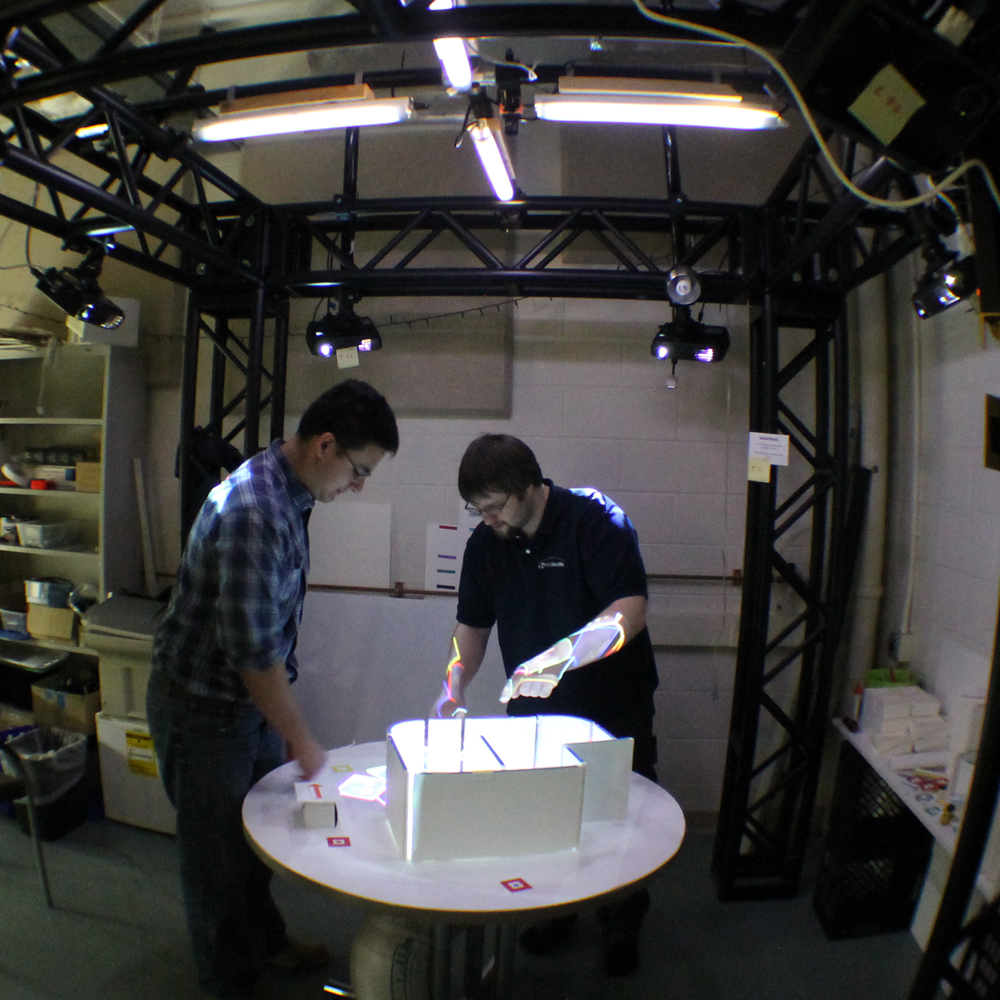
\includegraphics{photos/ian_matt_contraption_frame.jpg}}
\hfill
\resizebox{!}{\picheight}{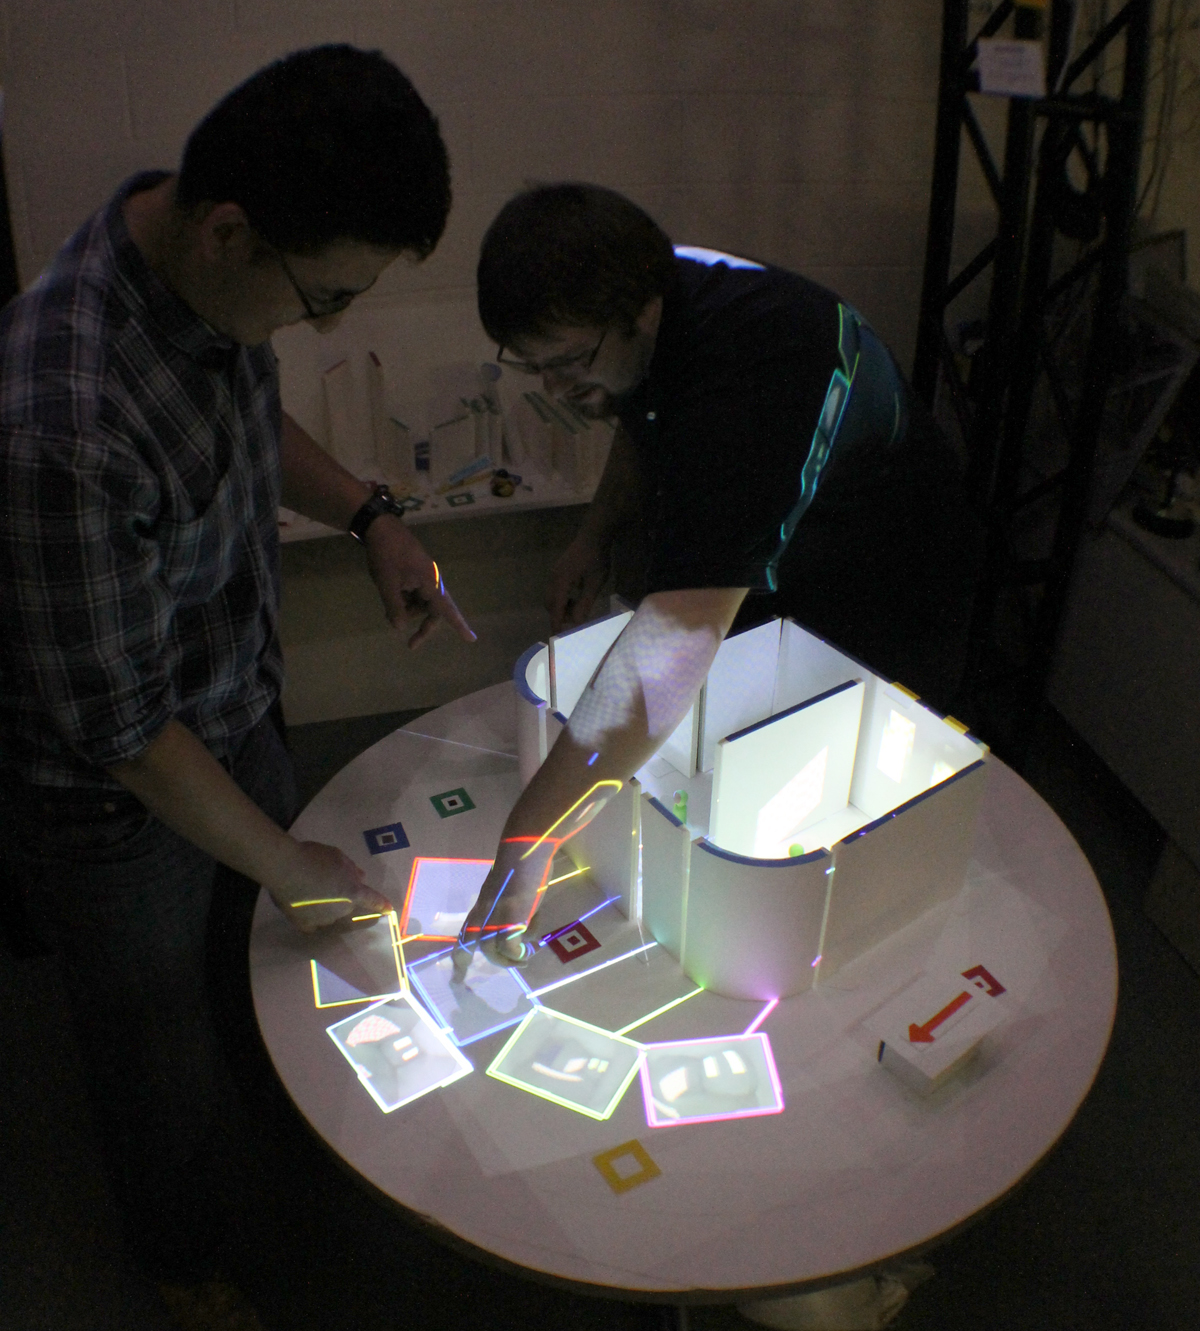
\includegraphics{photos/ian_matt_pointing.jpg}}
%\resizebox{\picheight}{!}{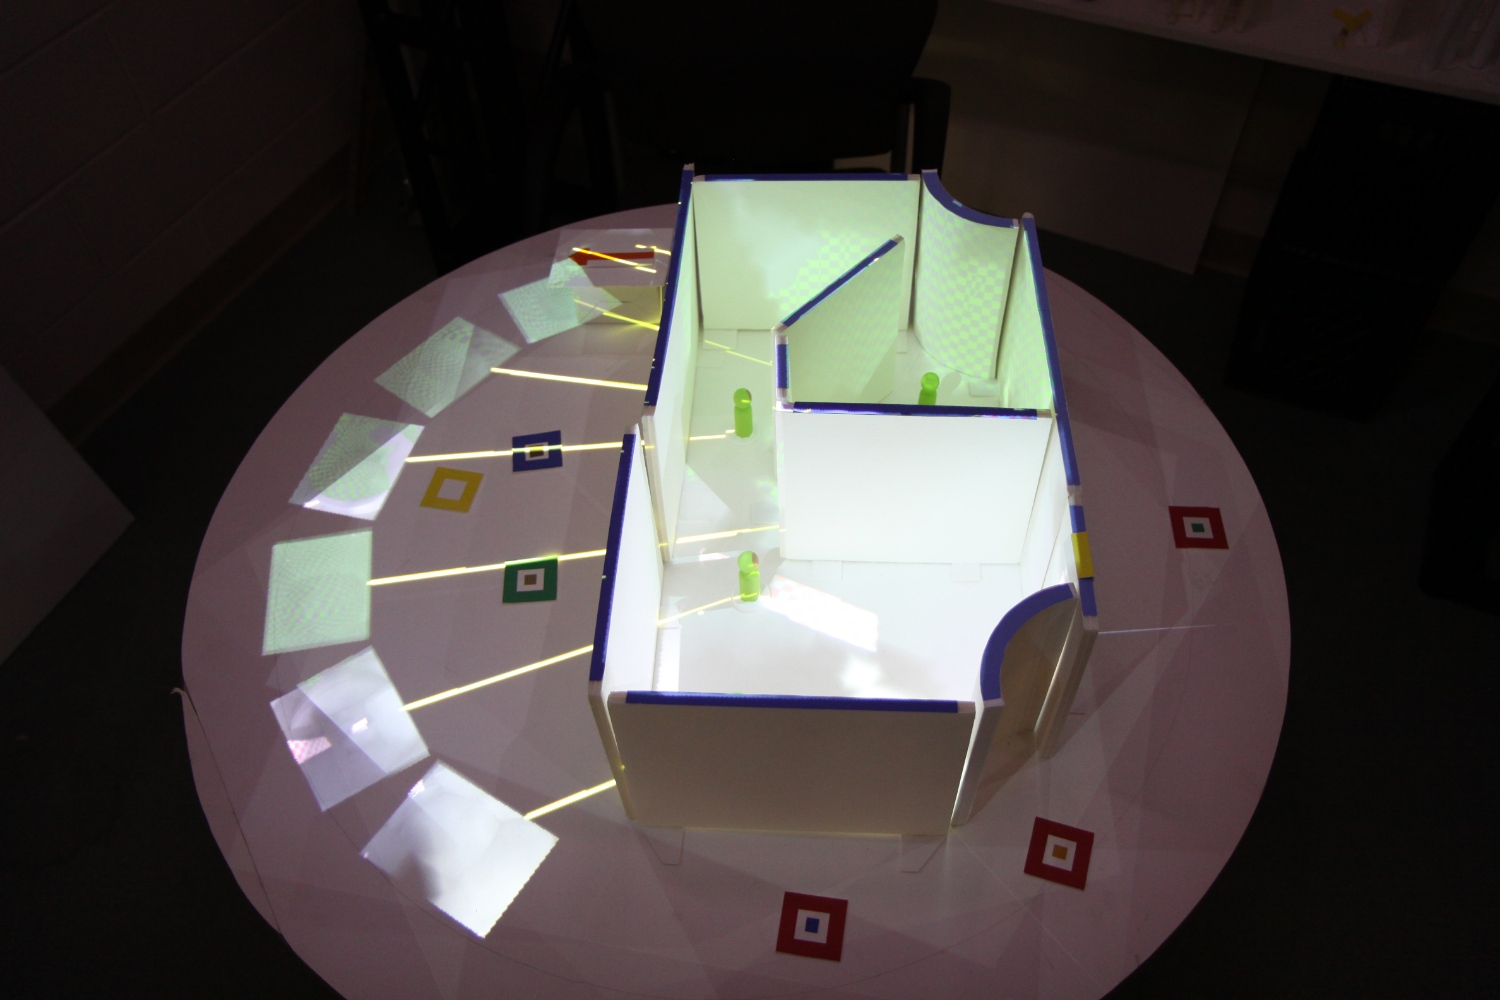
\includegraphics{photos/overhead_teaser.JPG}}
%\resizebox{\picheight}{!}{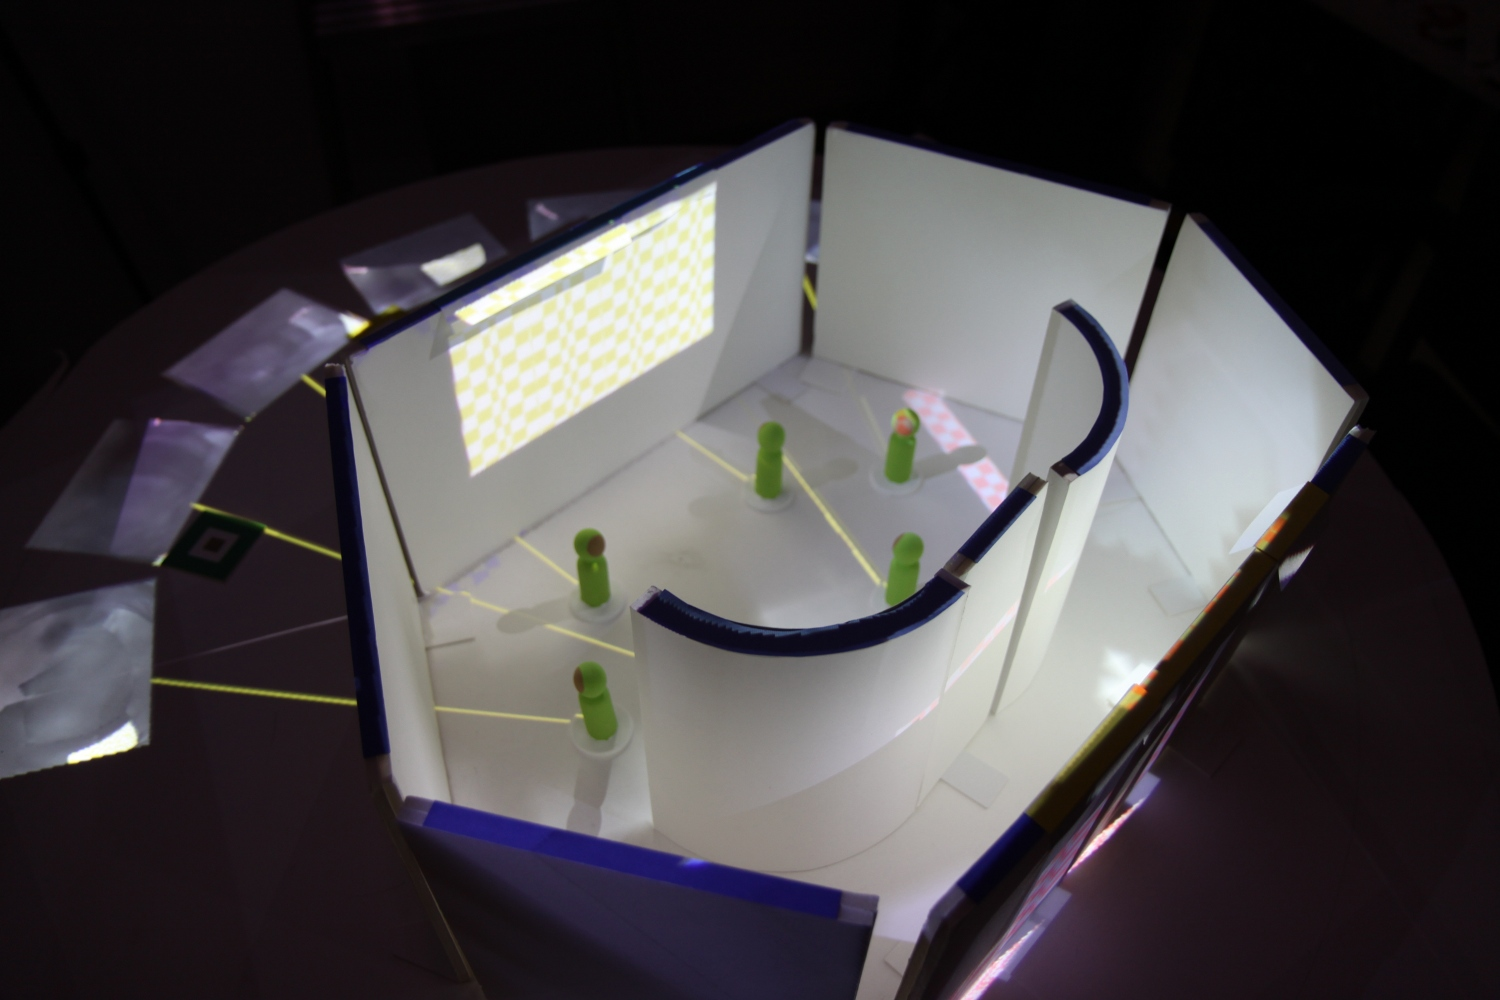
\includegraphics{photos/overhead_teaser2.JPG}}
\hfill
\resizebox{\picheightb}{!}{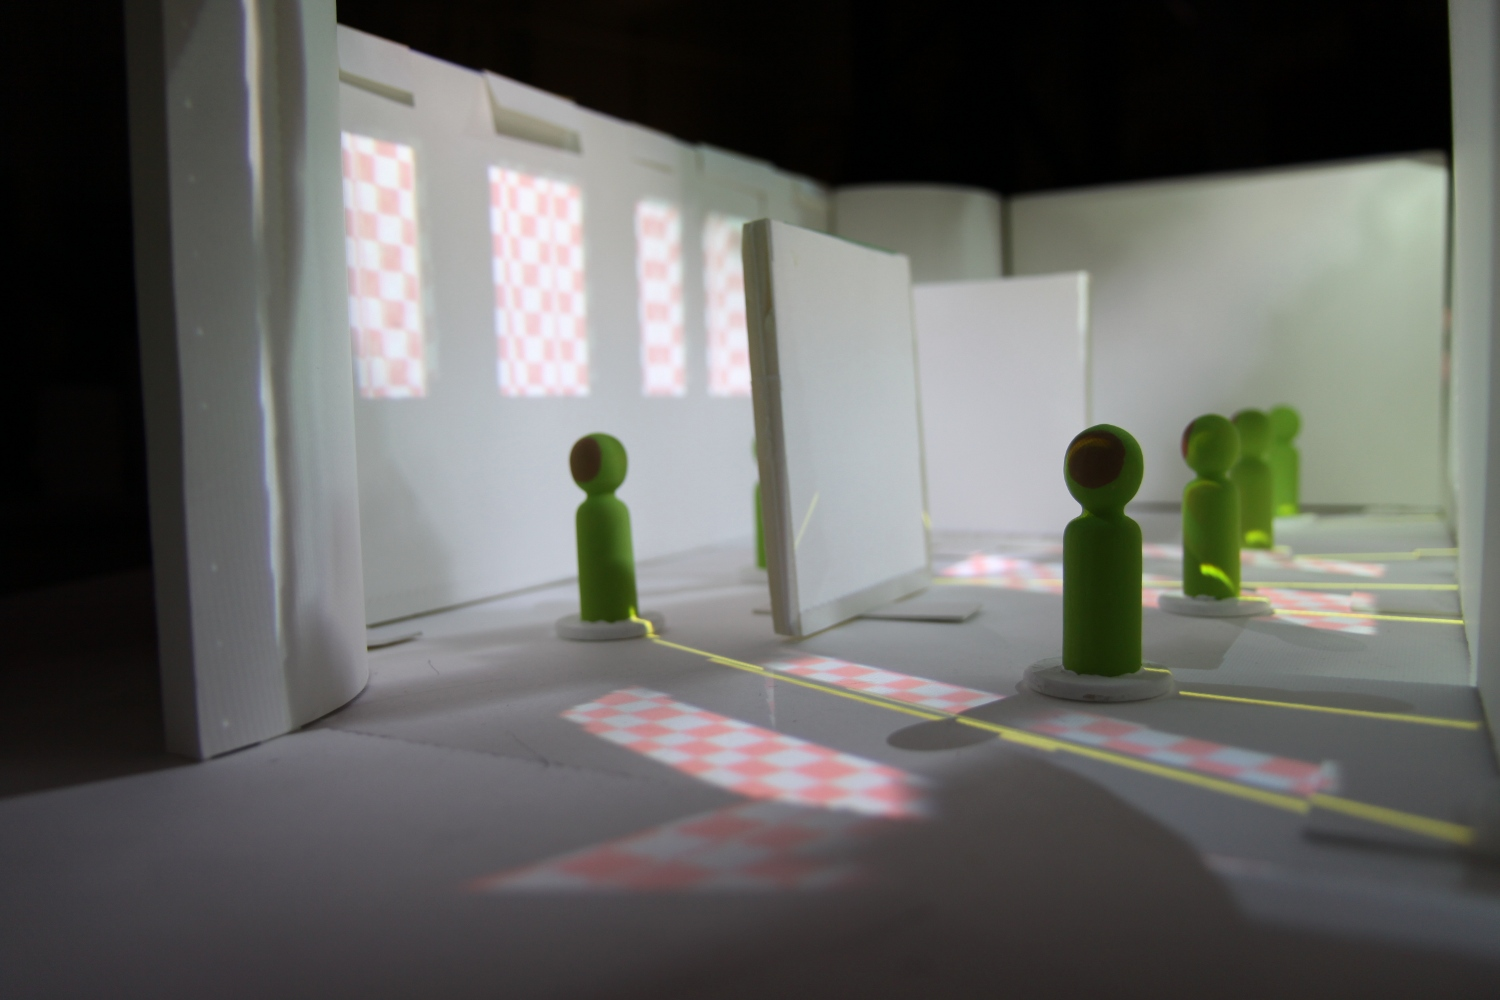
\includegraphics{photos/peeps_teaser.JPG}}\\

\vspace{-2.75in}
\hspace*{1in} \hfill 
\resizebox{\picheightb}{!}{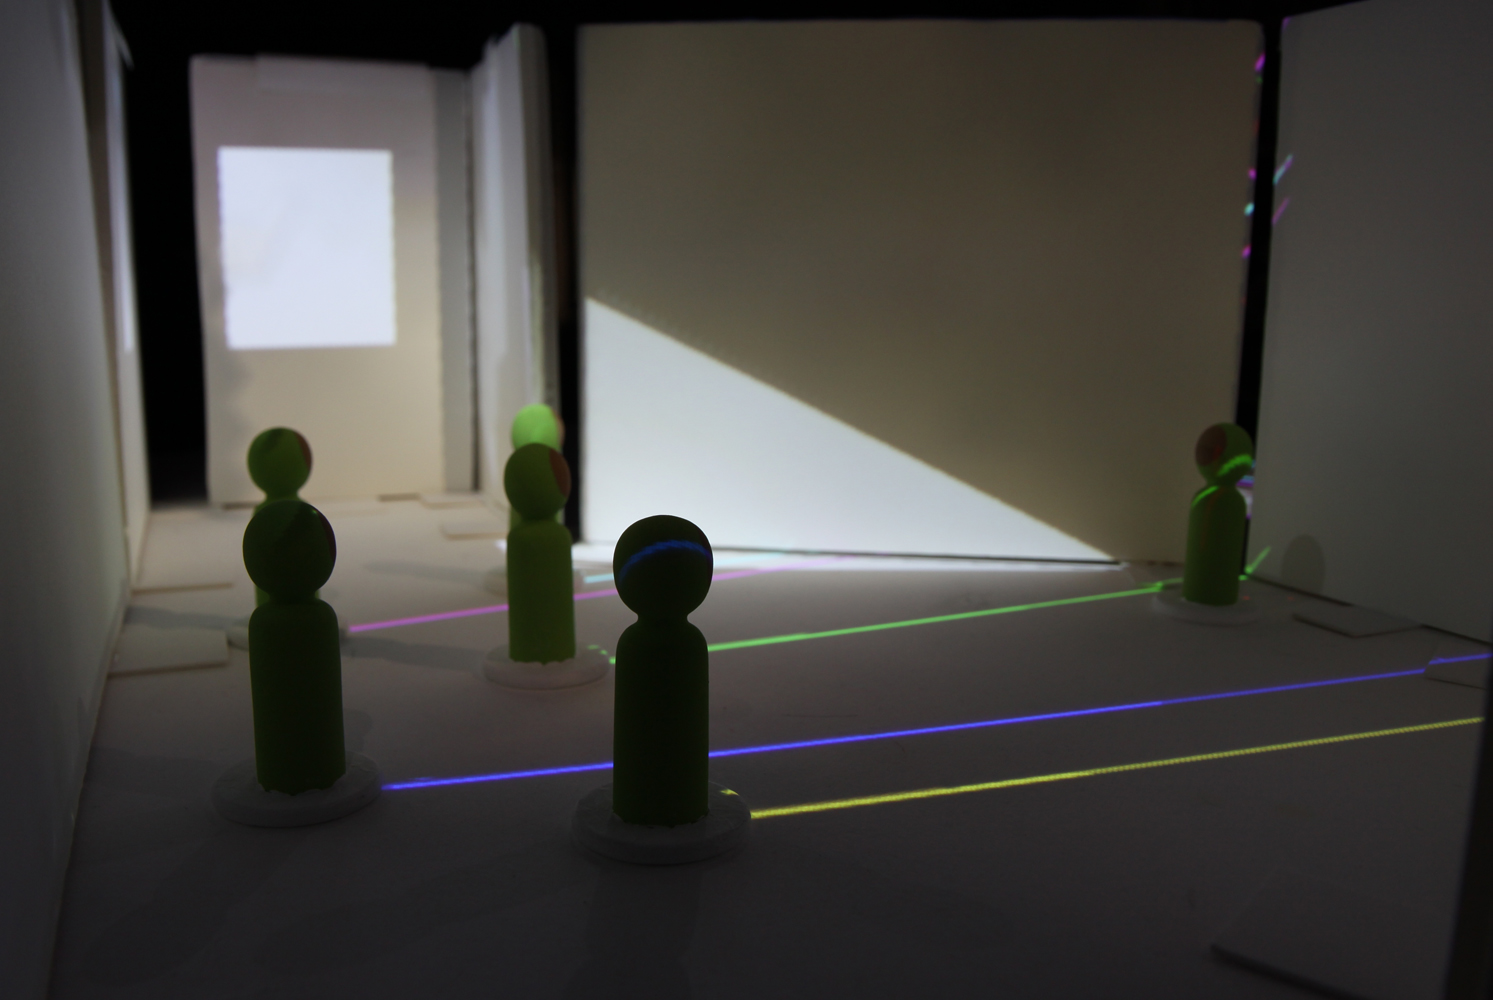
\includegraphics{photos/classroom_closeup.jpg}}\\
%\resizebox{\picheight}{!}{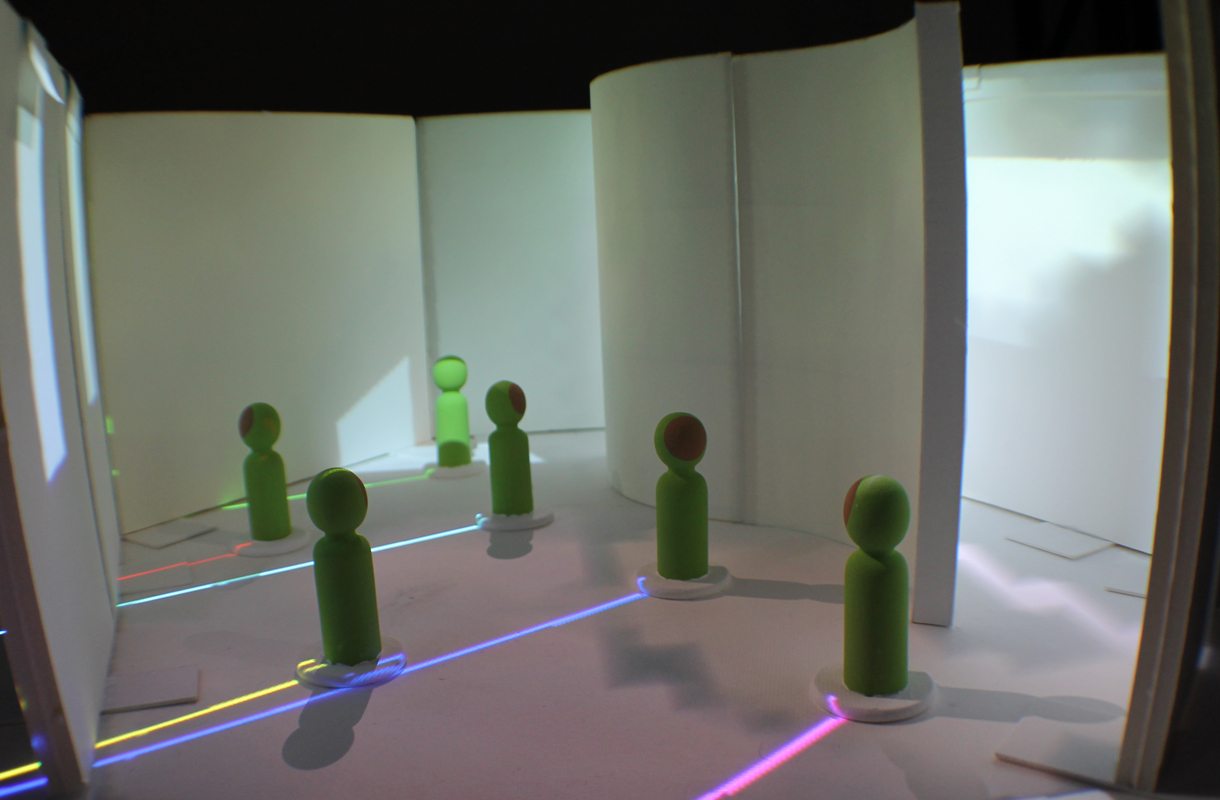
\includegraphics{photos/museum_fisheye.jpg}}

\vspace{1.2in}
%\vspace{-0.1in}
\caption{We provide tokens for users to specify locations of interest.  Renderings are provided for each glare avatar around the side of the table.}
\vspace{-0.15in}
\label{FIGURE:teaser}
\end{figure*}

%%%%%%%%% BODY TEXT
\section{Introduction}

%\subsection{Tabletop system}

%We have extended a
%For our system 
%we use a Tangible User Interface, TUI, for

%For our system we use a Tangible User Interface, TUI, for
%architectural daylighting design.  The system allows skectching an
%architectural model with physical primitives (see Figure
%\ref{FIGURE:teaser}).  In order to create a complete model, a user
%places wall primitives, window primitives and a north arrow on the
%table.  In addition primitives to specify wall color, ceiling color,
%floor color and glare sensors are available.


We have developed a Tangible User Interface for visualization of
customized architectural daylighting simulations.  The user physically
constructs of a small scale architectural model with physical walls
primitives (see Figure~\ref{FIGURE:teaser}), adding tokens to mark
windows, specify surface materials and the surrounding environment
(north orientation).  
%In order to create a complete model, a user
%places wall primitives, window primitives and a north arrow on the
%table.  
%
Additionally, small ``people'' token are placed within the model to
identify and measure the directional illumination within the simulated
volume.

%In addition primitives to specify
%wall color, ceiling color, floor color and glare sensors are
%available.

For each simulation, a single calibrated overhead camera captures the
scene.  Normally to capture 3-D geometry at least 2 calibrated cameras
are required. By having a single camera directly above the table and
indicating wall height with a colored indicator on the wall top, we
are able to infer the 3-D geometry.  
%Once the 3-D geometry has been
%captured a closed 3-D mesh is generated using the algorithm described
%in Cutler\cite{aag201015}.

Lighting is calculated for the mesh on a specified time and day.  A
variation on image spaced photon mapping \cite{mcguire09imagespace} is used to
calculate the light in the space and each plane of the model is
rendered.

Our multi-projector system is run in a master slave configuration.
The master sends each of the renderings to each process on the slave
computers.  Each process renders the geometry of the scene with its
generated textures overlaid on each wall.  Each projector projects a
portion of the scene onto the physical geometry using projector
blending.

The system allows users to make physical sketches with foam core walls
in three heights: 5", 8" and 10".  Window markers are available in two colors
to create taller and shorter windows.  Once a design has been completed, 
the user can request a time and date to be simulated.  In a normal workflow,
the user will try several times, make modifications to the room and iterate 
until they are satisfied with the design.  We ran a user study where users
had difficulty discerning what areas of the room  were too bright, too dark or 
had glare problems.  Users have also expressed interest in having options for 
more complicated lighting options.  For this reason we updated the physical
controls of the system, the visualization modes, and window materials.

\subsection {Our Contributions}


The contributions we present in this paper are:

\begin{itemize}
\item Present a false color visualization for use in analyzing areas of over and under-illumination.
\item Provide tokens for users to place in a physical representation of a room to analyze \emph{glare}: difficulty seeing due to the presence of bright light in a person's view.
\item Provide the option for users to put complicated window geometry into their model while providing them with both a high detail rendering and accurate lighting information.
\end{itemize}


\subsection{Daylighting simulation}
Rendering daylighting requires another level of complexity than
rendering with point light sources.  Our simulation divides the direct
light computation from the global illumination which is computed using
photon mapping.  There are four standard sky types that are used for
daylighting simulation: clear sky, intermediate sky, turbid sky and
overcast sky \cite{international1994spatial,perez1990modeling}.  Each
of these models is based upon having the illuminance value for the
zenith \cite{Karayel1984283} and measurements of the illuminance for
the ground plane.  For our renderings, we have used the CIE clear sky
model.


\section{Related Work}

\subsection{Tangible User Interfaces}


One of the earliest TUIs was developed by Ishii and Ullmer
\cite{Ishii97tangiblebits}.  They allowed users to manipulate digital
information by controlling their system with physical icons.  Jacob
extended the TUI by projecting information on movable physical
objects \cite{Jacob01atangible}.  The ``bricks" system was the first interface
to allow multiple physical controls in a TUI system to be used together to expand
information shown \cite{223964}.  The JUMP tool continued to
improve controls for a TUI by using a variety of tokens in a projector
camera system to allow users to switch between multiple architectural
documents to rectify them\cite{1268540}. We also allow users to switch between
layers of data: a daylighting rendering and a false color visualization mode of the
same model.  The URban Planning system provided an interface that
enabled users to see how buildings would cast shadows on each other\cite{Underkoffler:1999:ULW:302979.303114}.
Our system also displays daylighting in architecture but is designed
to simulate interior light.
%\fbox{more analysis}





\subsection{Projector Camera Interfaces}

%Need to tie these in better?


Projector Camera systems have been used in a variety of ways to
communicate information. Mitsugami used multiple moving projectors
together to produce a single image\cite{MitsugamiUK07}.  While we are
using a system with six projectors, dynamic alignment of projectors is
unnecessary because our projectors' positions are static.  Barnum
created a projector camera system which used falling water drops as a
projection surface\cite{Barnum09aprojector-camera}.

Projector Camera systems are well suited to project 3-D
information. Amano printed a normal map on paper and then used a
projector camera system to project an image of the model with a
light's location changing\cite{DBLP:conf/cvpr/Amano12}.  While their
system only projects on a single 2-D surface our system projects 2-D
planes onto a 3-D model to show a 3-D lighting simulation.  Gartska
used a Kinect to track a user's head position and
orientation\cite{Garstka_Peters_2004}.  Based on this information, a
projection of a 3-D image was changed so that it appeared the user
could move in relation to a 3-D object.  Menk \cite{menkandkoch} projected
3-D information onto a colorless 3-D model while taking into account
ambient light.  We also simulate light in a virtual model and project
it onto a real surface but Menk was incorporating the actual
environment on a real physical geometry whereas we are running a full
daylight simulation on a scale model of a space.

Projecting \emph{Spatially Immersive} information on normal surfaces was first 
presented in The Office of the Future \cite{Raskar:1998:OFU:280814.280861}.  This work was extended in Shader Lamps\cite{Raskar:2001:SLA}.
Similarly to Raskar \cite{Raskar:2001:SLA} and Sheng \cite{sheng_TVCG}, 
our system projects information on neutrally colored physical primitives
to create a detailed rendering of a simulated space.  Our physical primitives
and rendering options provide unique extensions to their work.




\begin{figure*}[t]

\begin{center}
\newcommand{\picheight}{2.5in}
\resizebox{!}{\picheight}{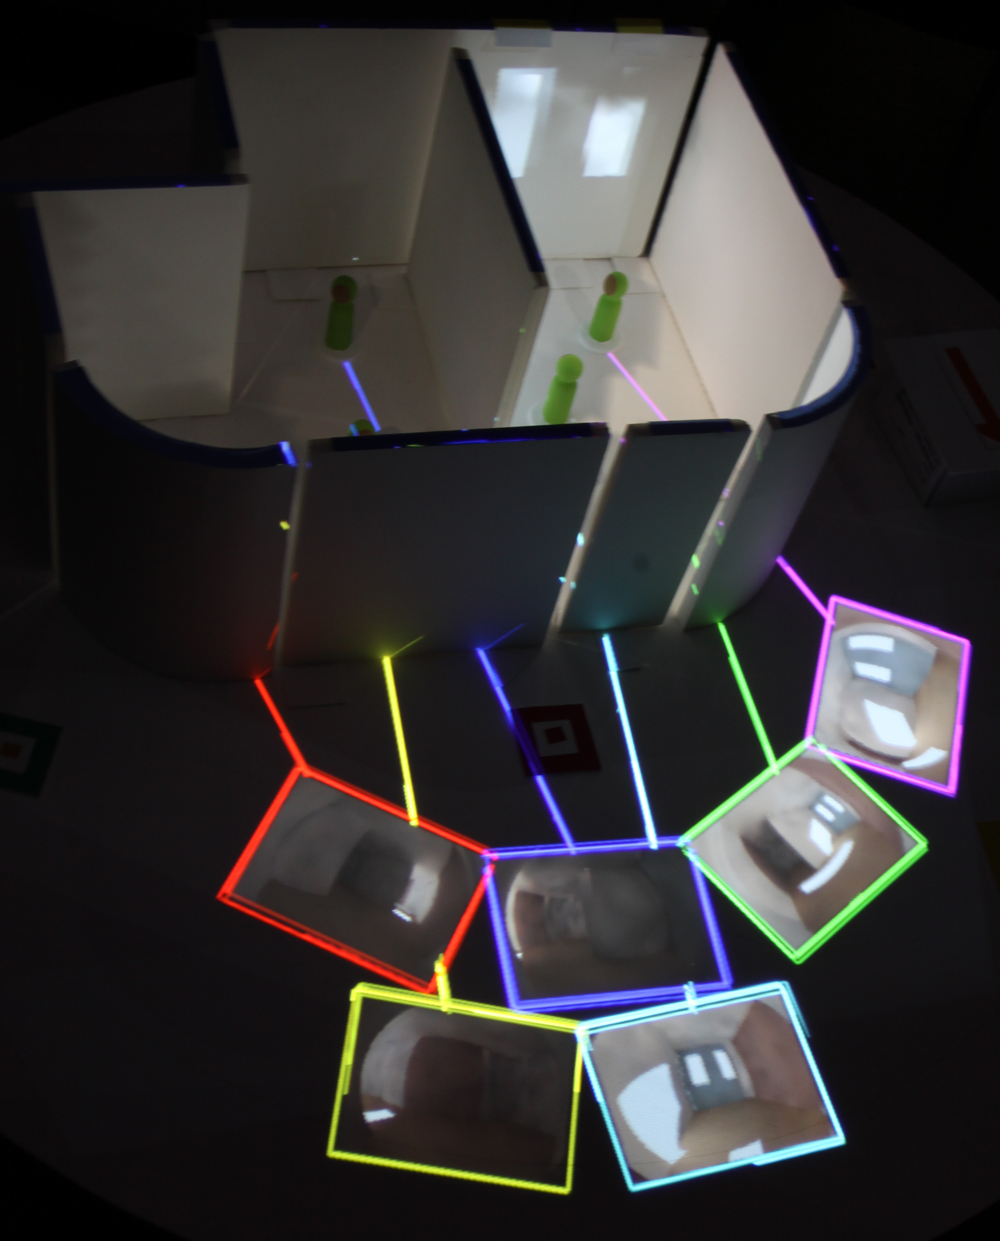
\includegraphics{photos/office_color.jpg}}
\resizebox{!}{\picheight}{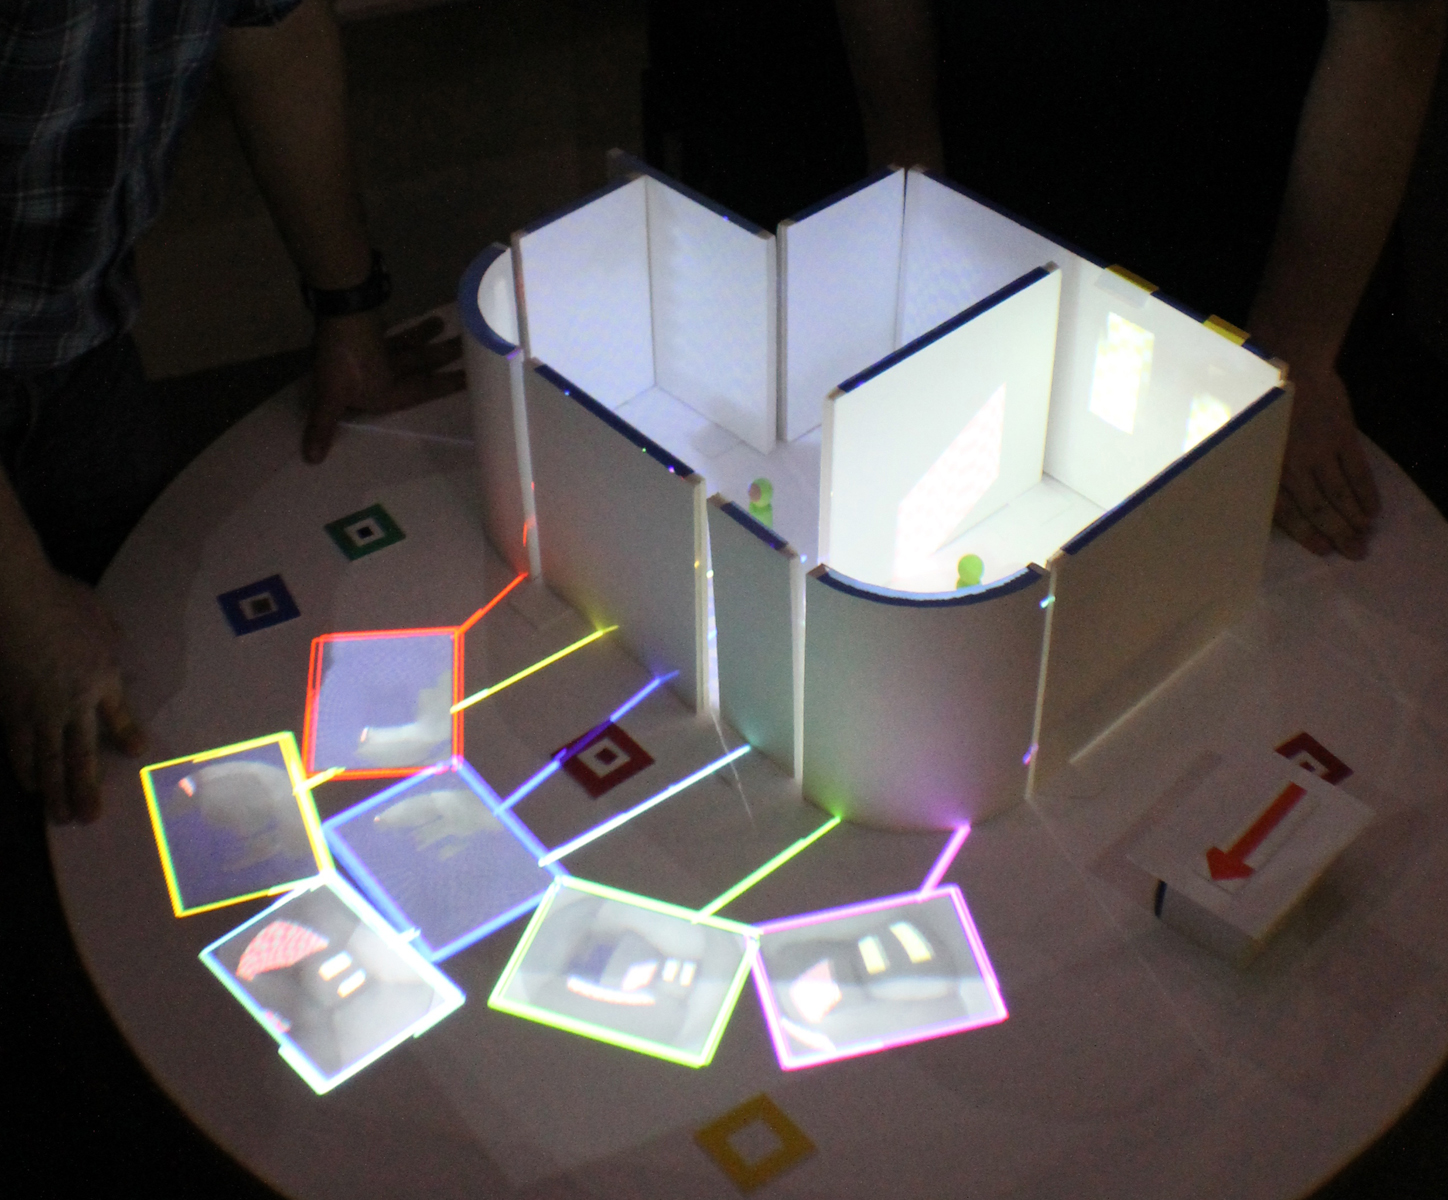
\includegraphics{photos/office_falsecolor.jpg}}
\end{center}
\vspace{-0.1in}
\caption{The most common problem users encountered in our user study
  was determining the areas that were too bright or too dark.  Our
  false color visualizations will help future user discern where the
  problem areas are.  The blue checkerboard is the under-illuminated
  area and the red checkerboard is the over-illuminated area.  The
  view point from each physical avatar are shown in
  Figure~\ref{FIGURE:fisheyes}.}
%\vspace{-0.15in}
\label{FIGURE:office_false_color}
\end{figure*}



\begin{figure*}[t]
\newcommand{\picwidth}{.95in}
%\resizebox{\picwidth}{!}{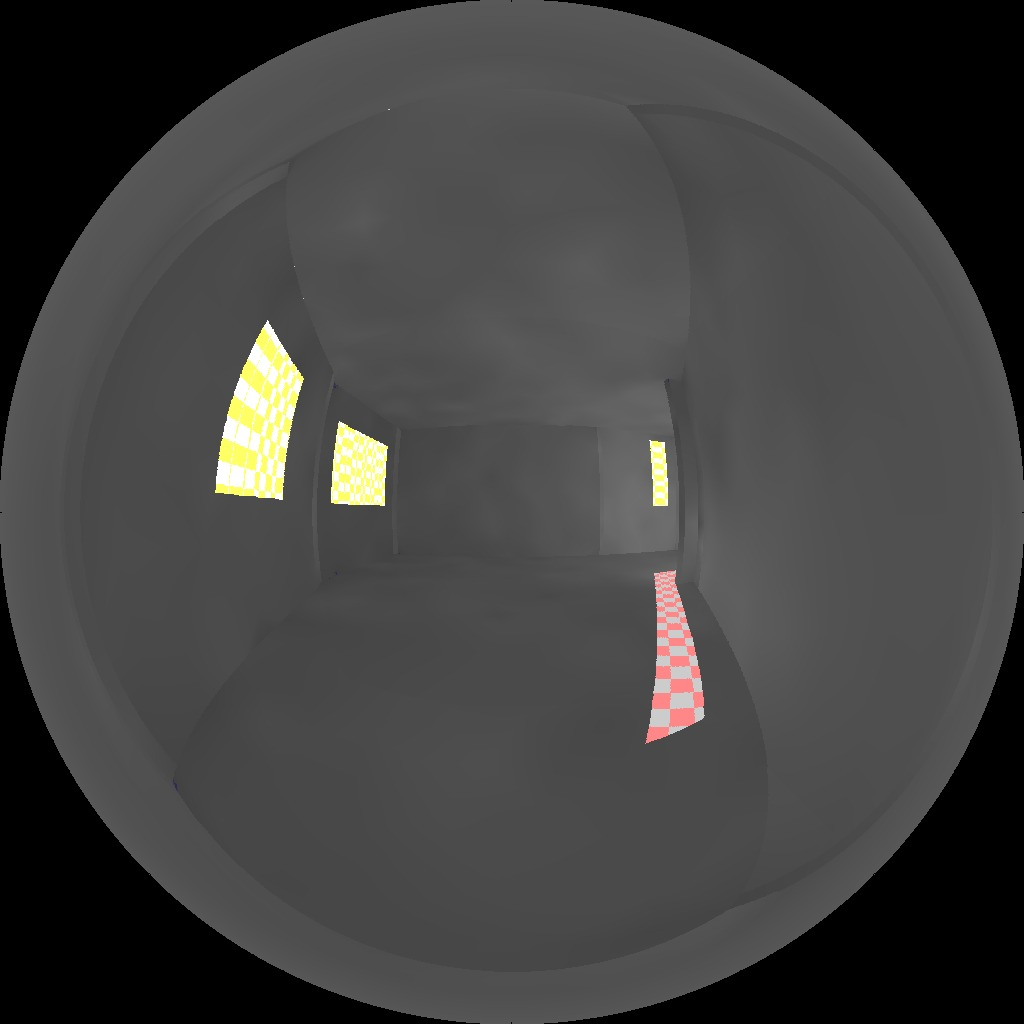
\includegraphics{wallfiles/classroom_12PM/surface_camera_VIEW_person0.jpg}}
%\resizebox{\picwidth}{!}{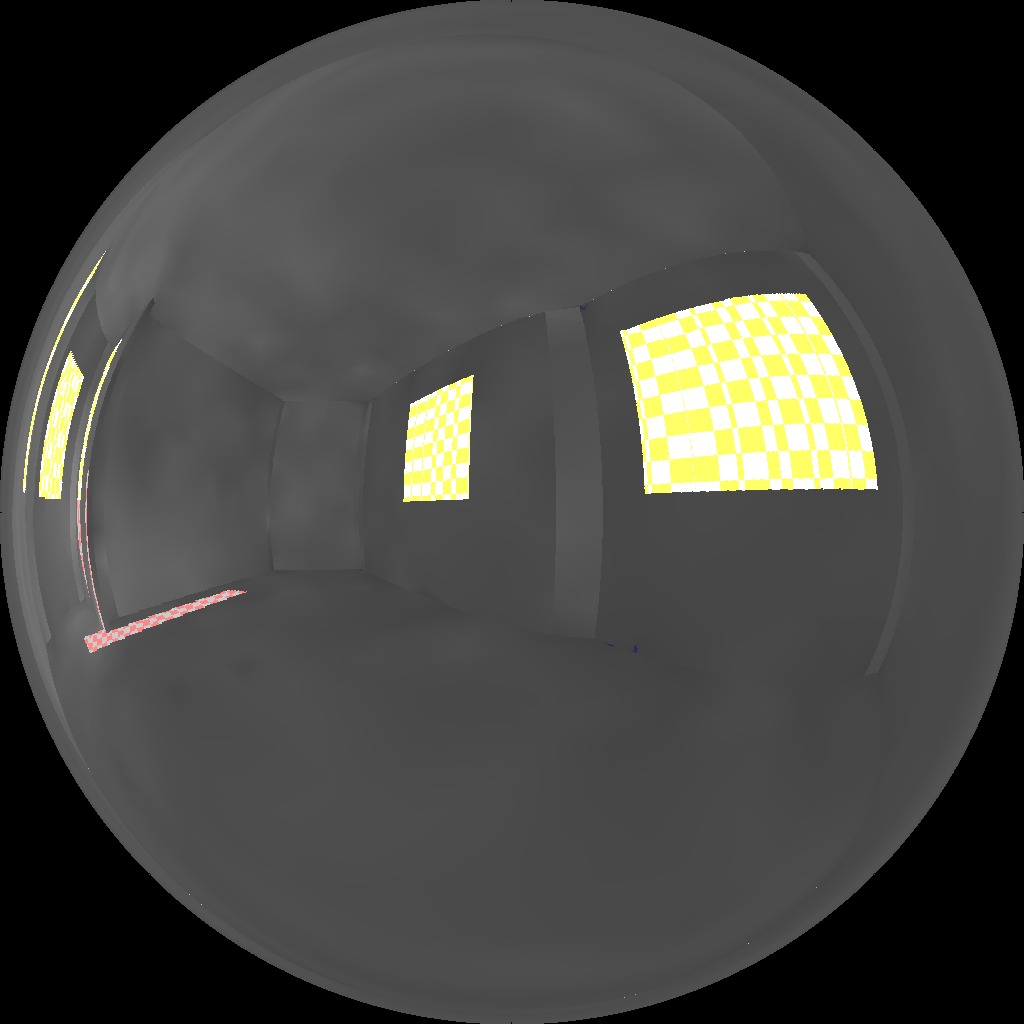
\includegraphics{wallfiles/classroom_12PM/surface_camera_VIEW_person1.jpg}}
%\resizebox{\picwidth}{!}{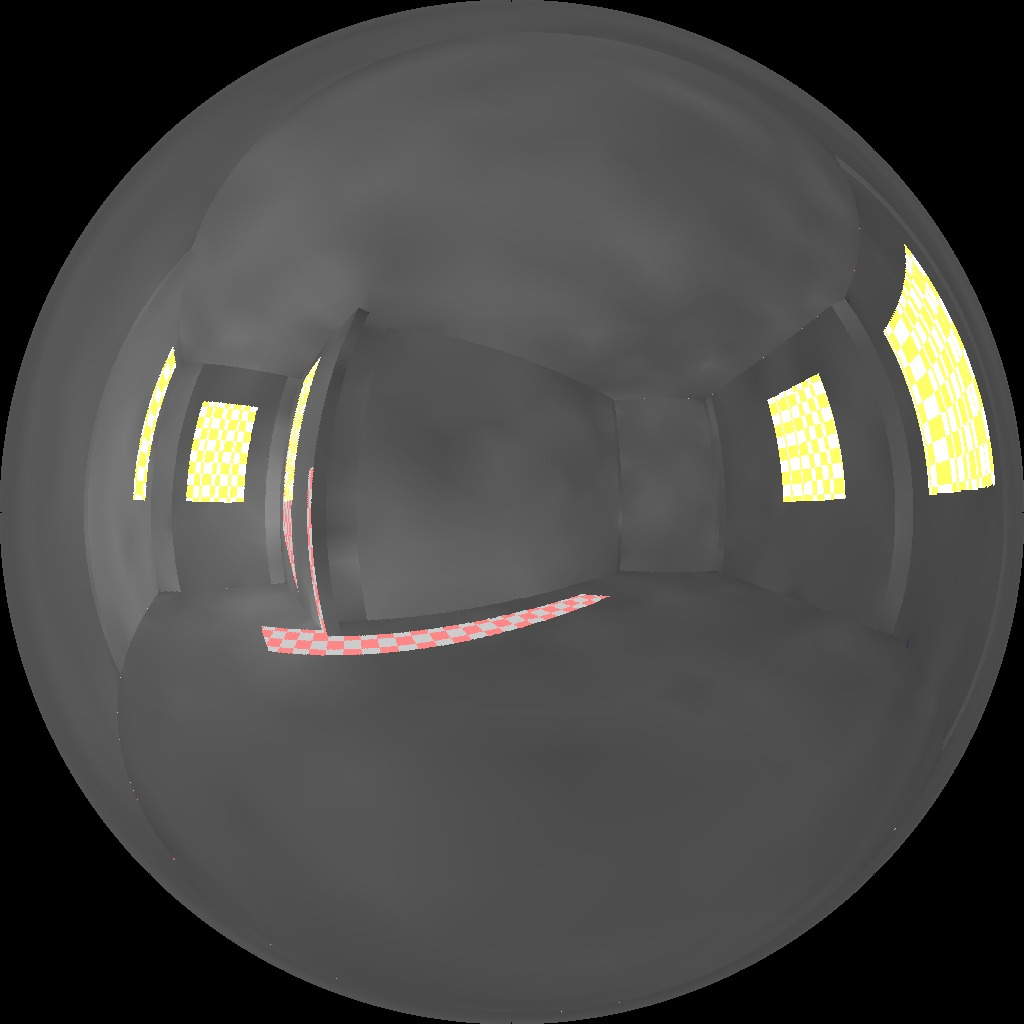
\includegraphics{wallfiles/classroom_12PM/surface_camera_VIEW_person2.jpg}}
%resizebox{\picwidth}{!}{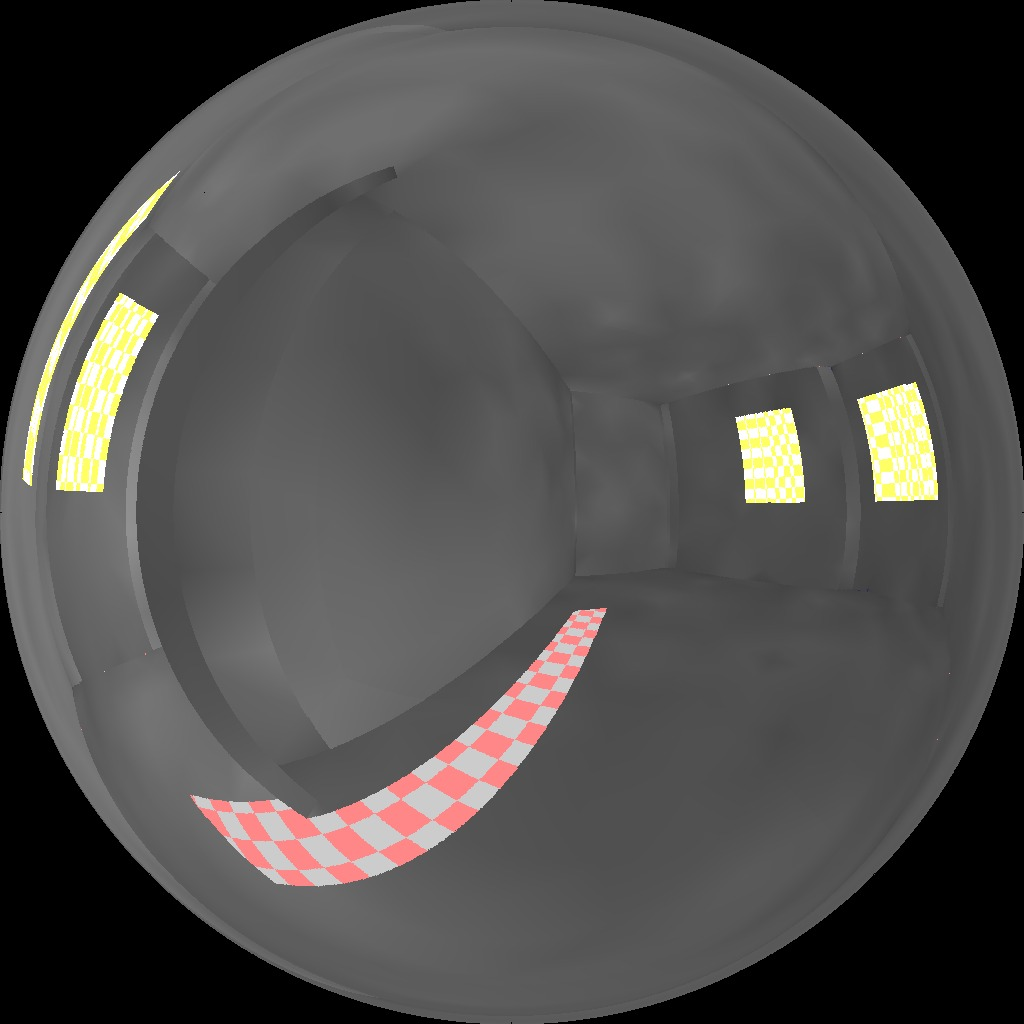
\includegraphics{wallfiles/classroom_12PM/surface_camera_VIEW_person3.jpg}}
%\resizebox{\picwidth}{!}{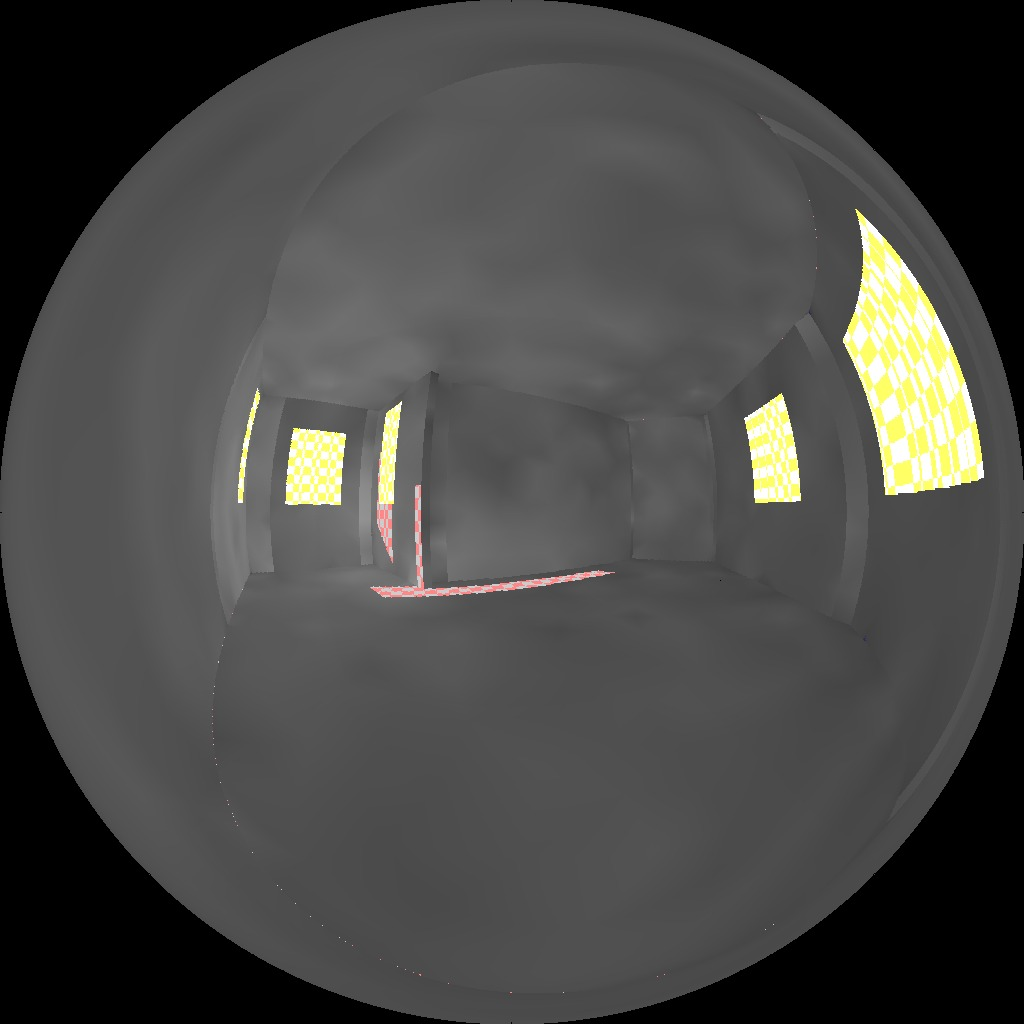
\includegraphics{wallfiles/classroom_12PM/surface_camera_VIEW_person4.jpg}}
%\resizebox{\picwidth}{!}{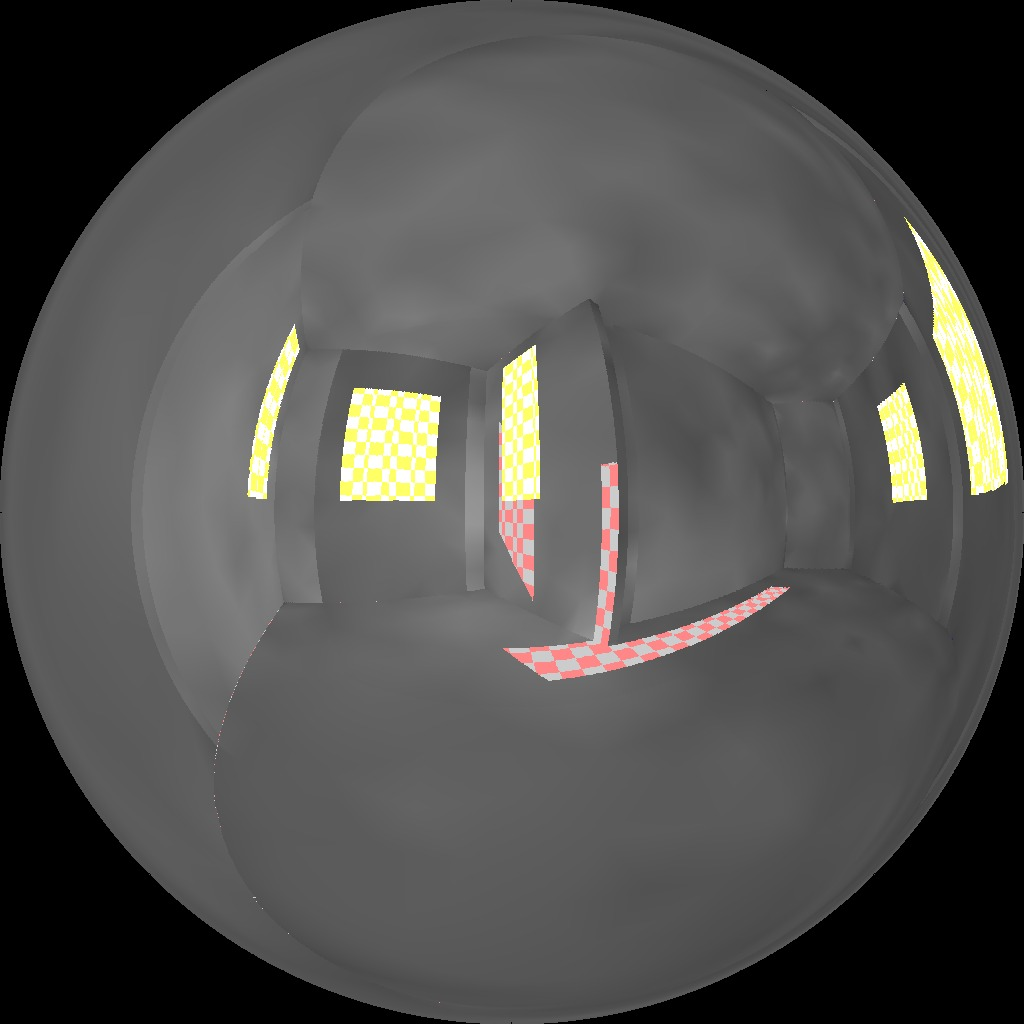
\includegraphics{wallfiles/classroom_12PM/surface_camera_VIEW_person5.jpg}}
%\\
%\resizebox{\picwidth}{!}{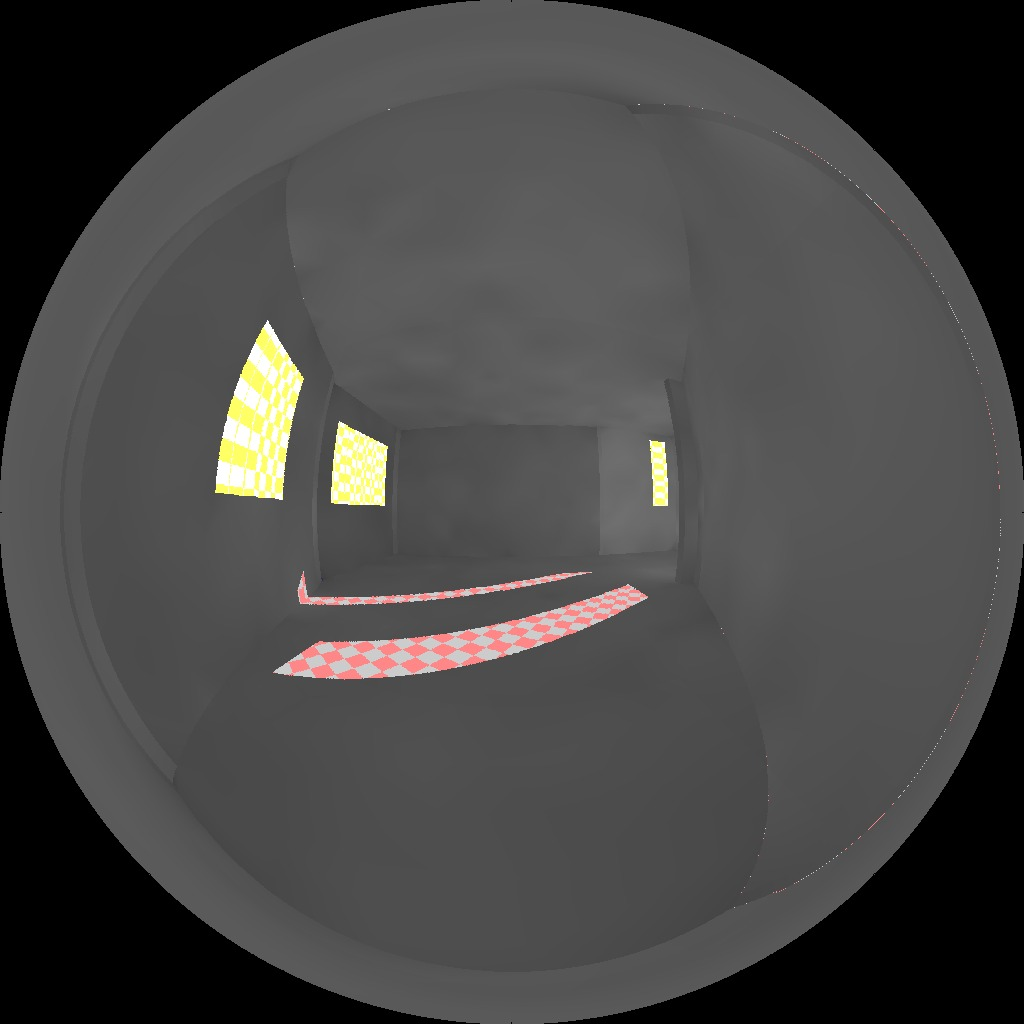
\includegraphics{wallfiles/classroom_2PM/surface_camera_VIEW_person0.jpg}}
%\resizebox{\picwidth}{!}{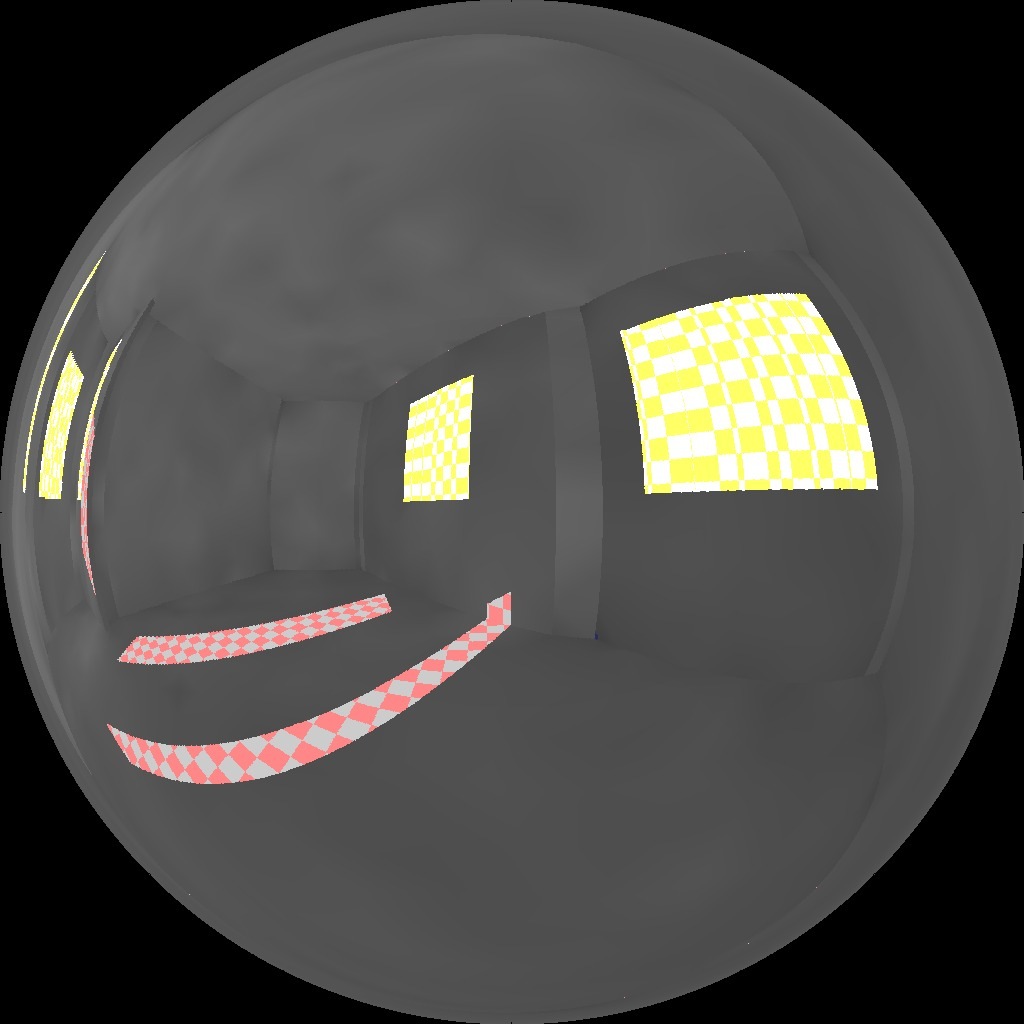
\includegraphics{wallfiles/classroom_2PM/surface_camera_VIEW_person1.jpg}}
%\resizebox{\picwidth}{!}{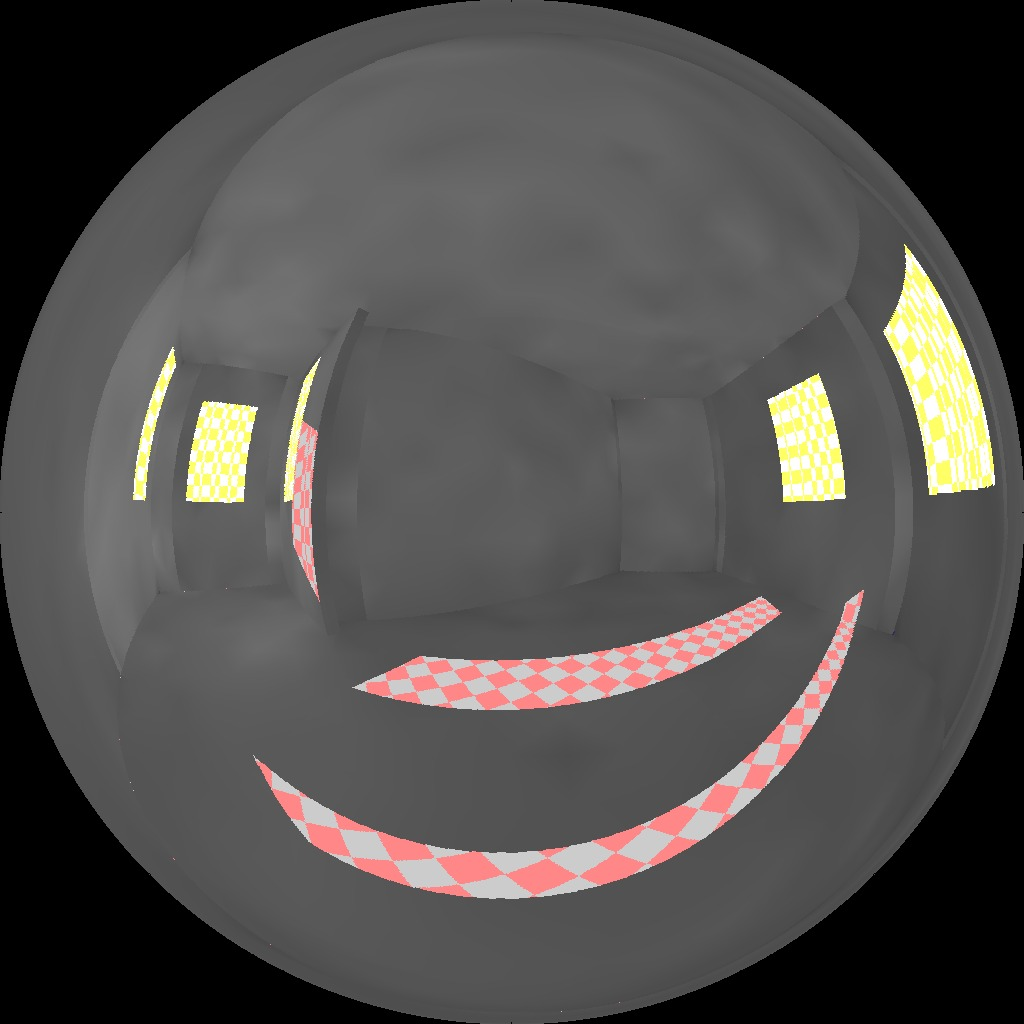
\includegraphics{wallfiles/classroom_2PM/surface_camera_VIEW_person2.jpg}}
%\resizebox{\picwidth}{!}{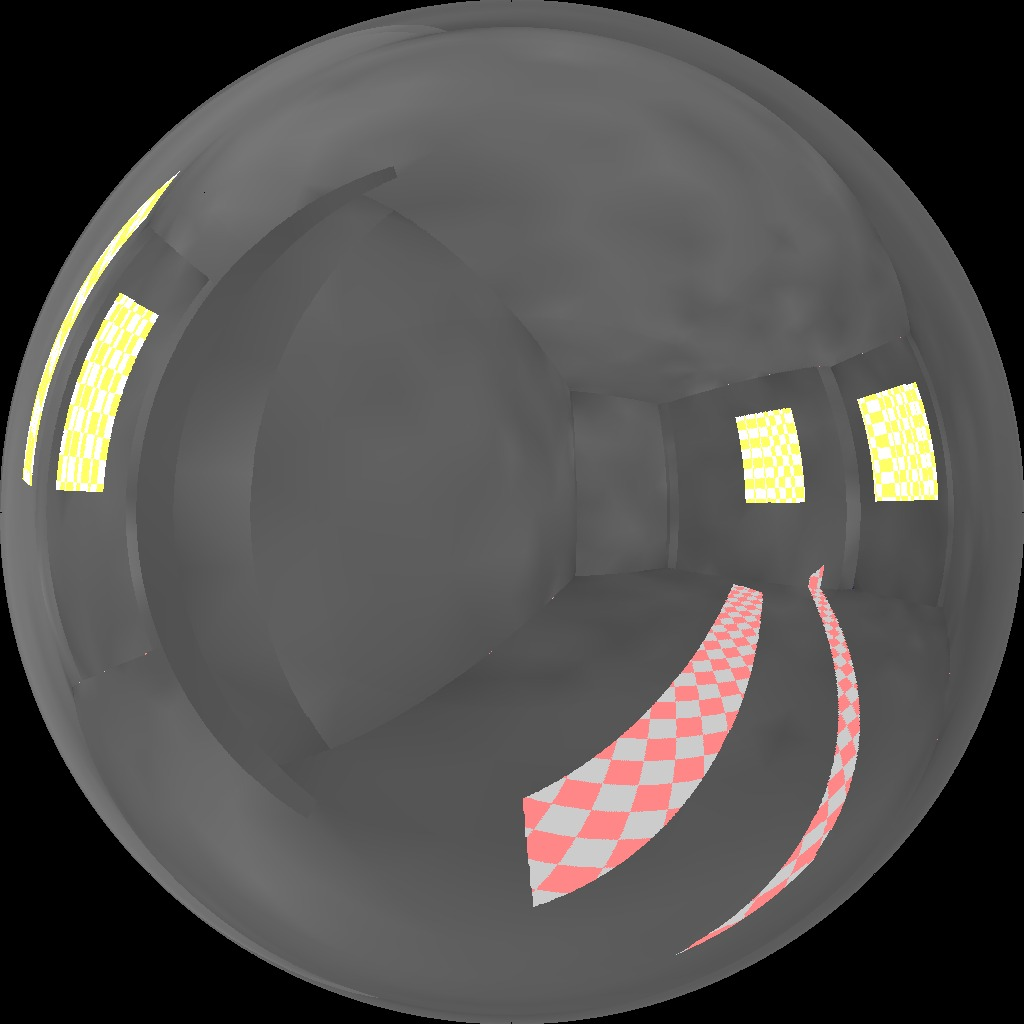
\includegraphics{wallfiles/classroom_2PM/surface_camera_VIEW_person3.jpg}}
%\resizebox{\picwidth}{!}{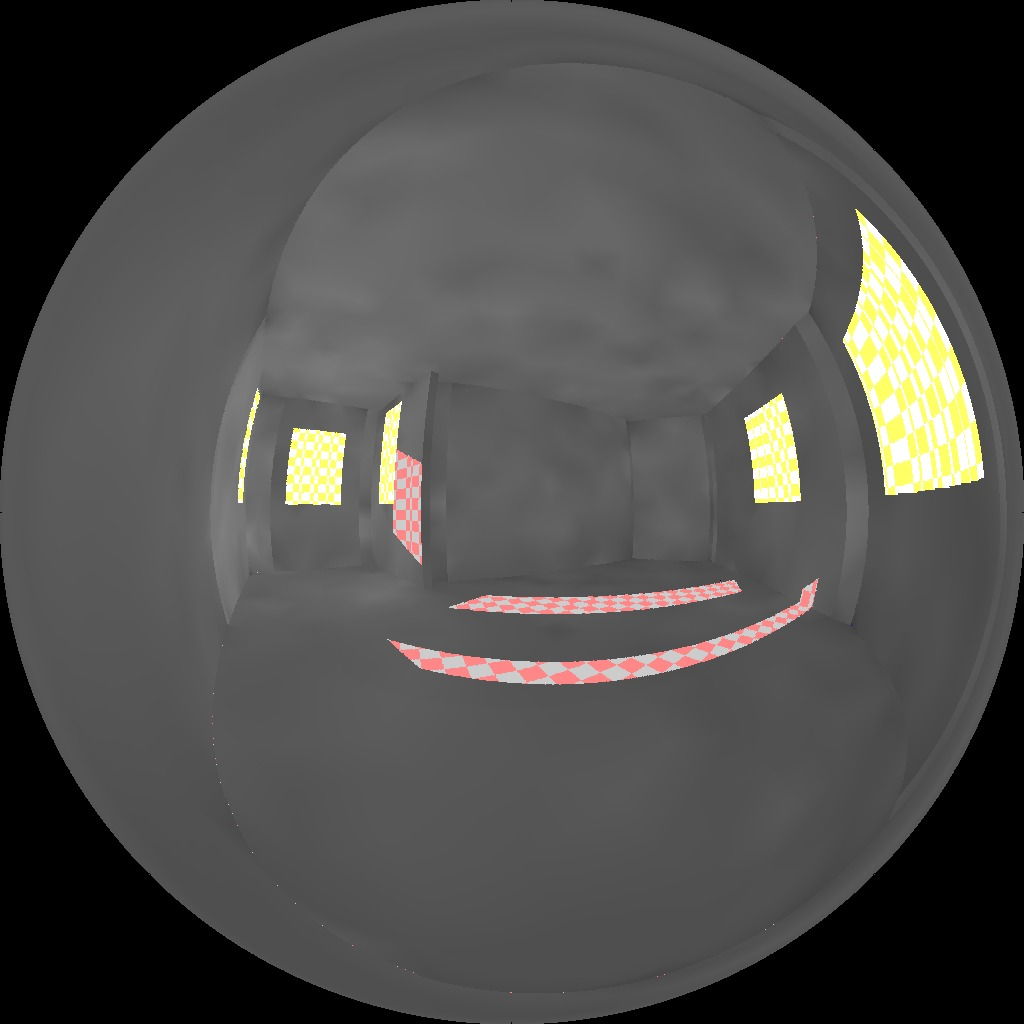
\includegraphics{wallfiles/classroom_2PM/surface_camera_VIEW_person4.jpg}}
%\resizebox{\picwidth}{!}{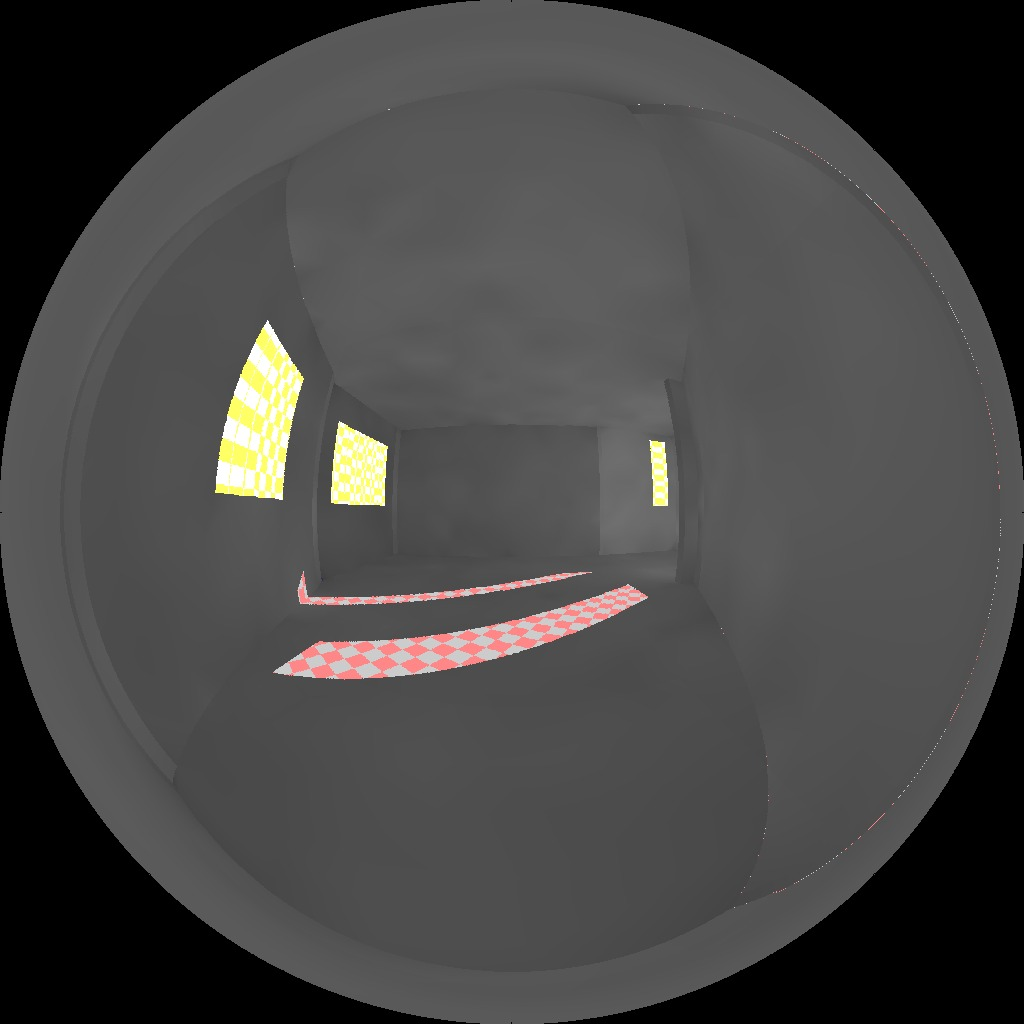
\includegraphics{wallfiles/classroom_2PM/surface_camera_VIEW_person5.jpg}}
%\vspace{-0.1in}
\resizebox{\picwidth}{!}{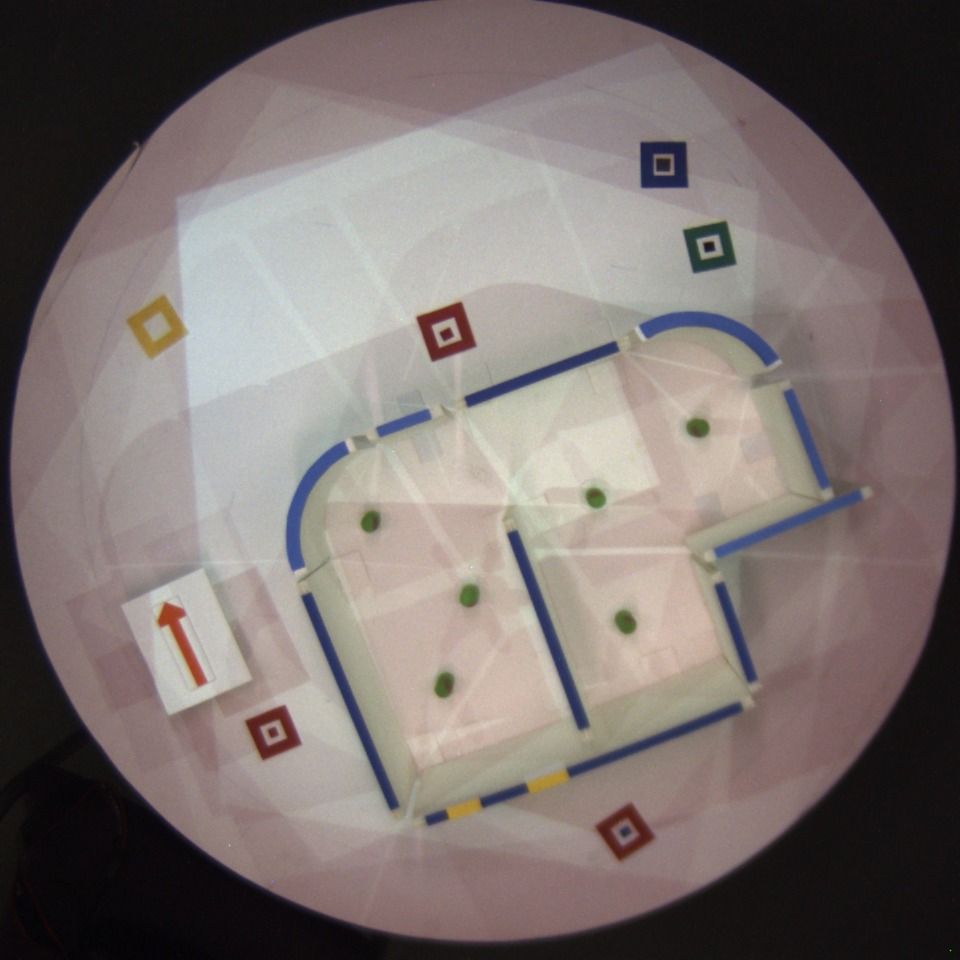
\includegraphics{wallfiles/mrc331/out.jpg}}
\resizebox{\picwidth}{!}{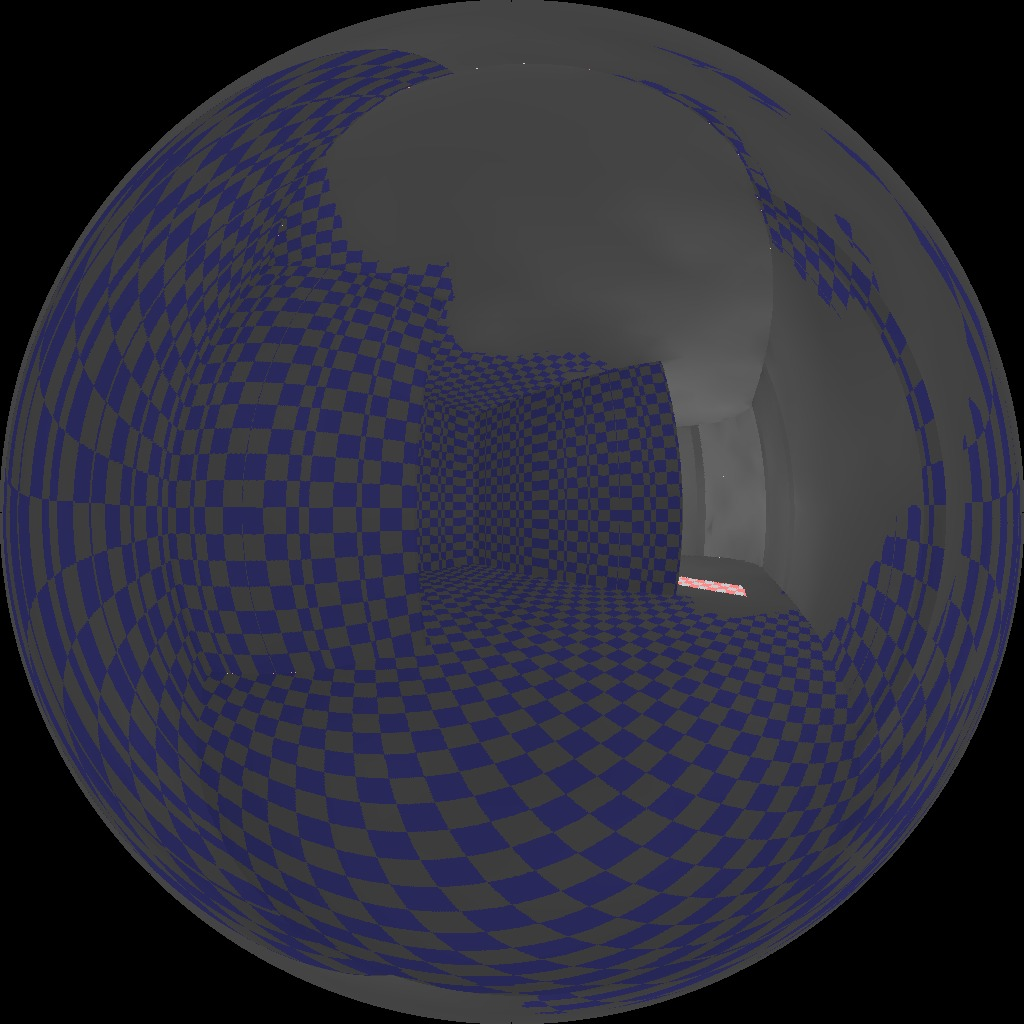
\includegraphics{wallfiles/mrc331/surface_camera_VIEW_person0.jpg}}
\resizebox{\picwidth}{!}{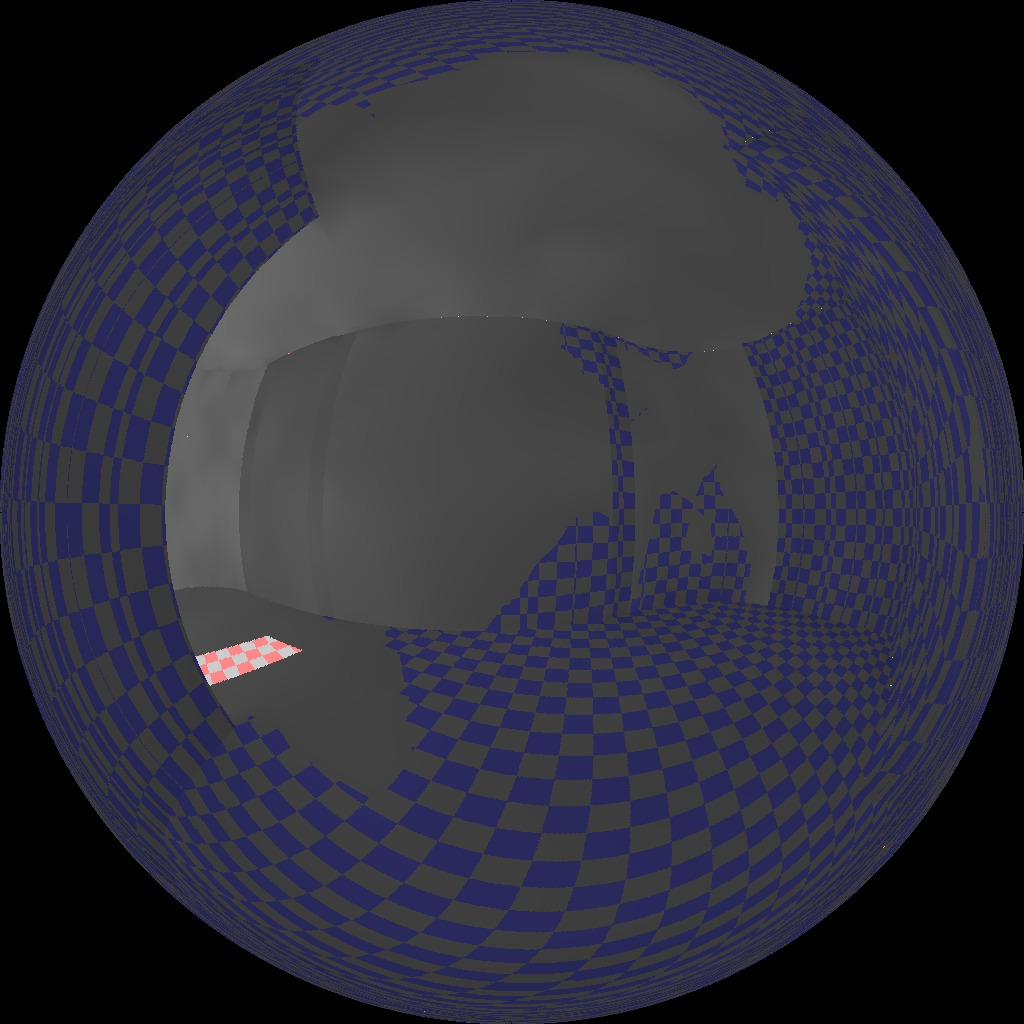
\includegraphics{wallfiles/mrc331/surface_camera_VIEW_person1.jpg}}
\resizebox{\picwidth}{!}{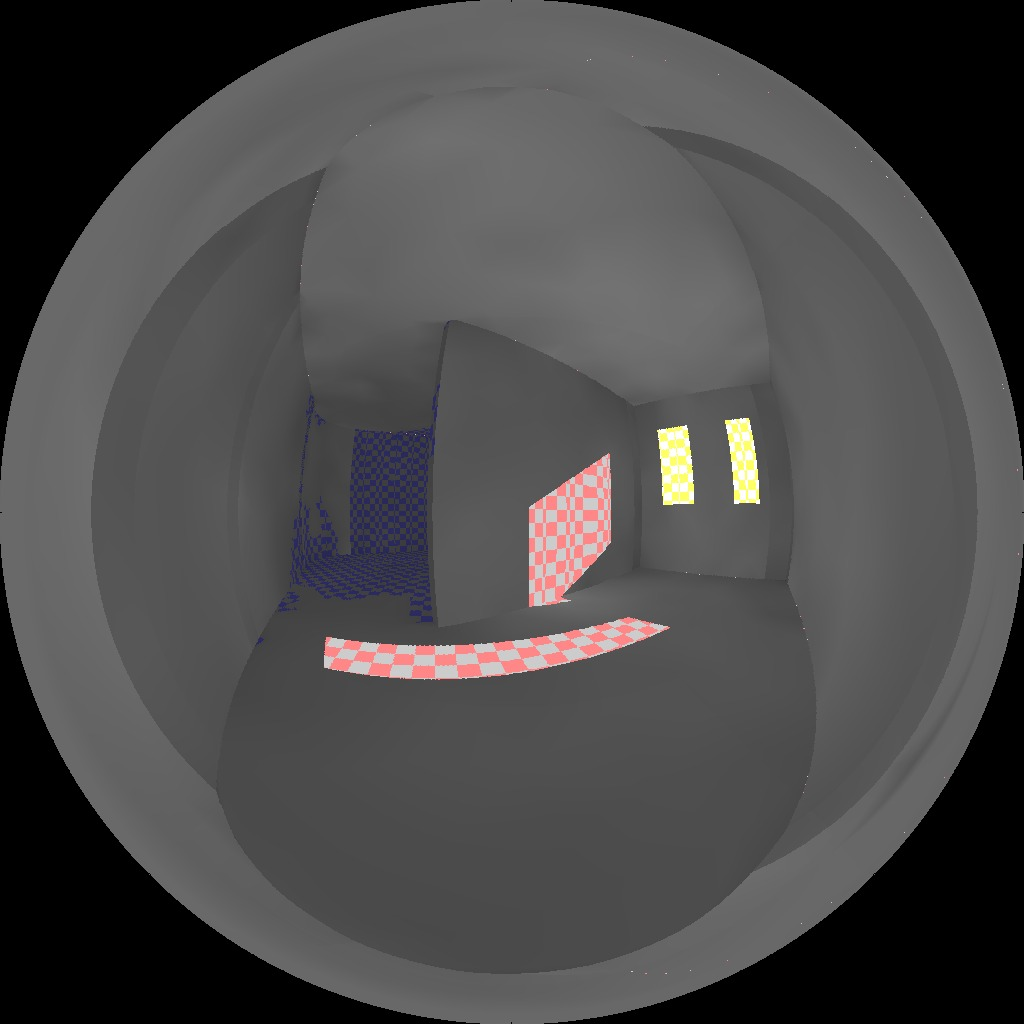
\includegraphics{wallfiles/mrc331/surface_camera_VIEW_person2.jpg}}
\resizebox{\picwidth}{!}{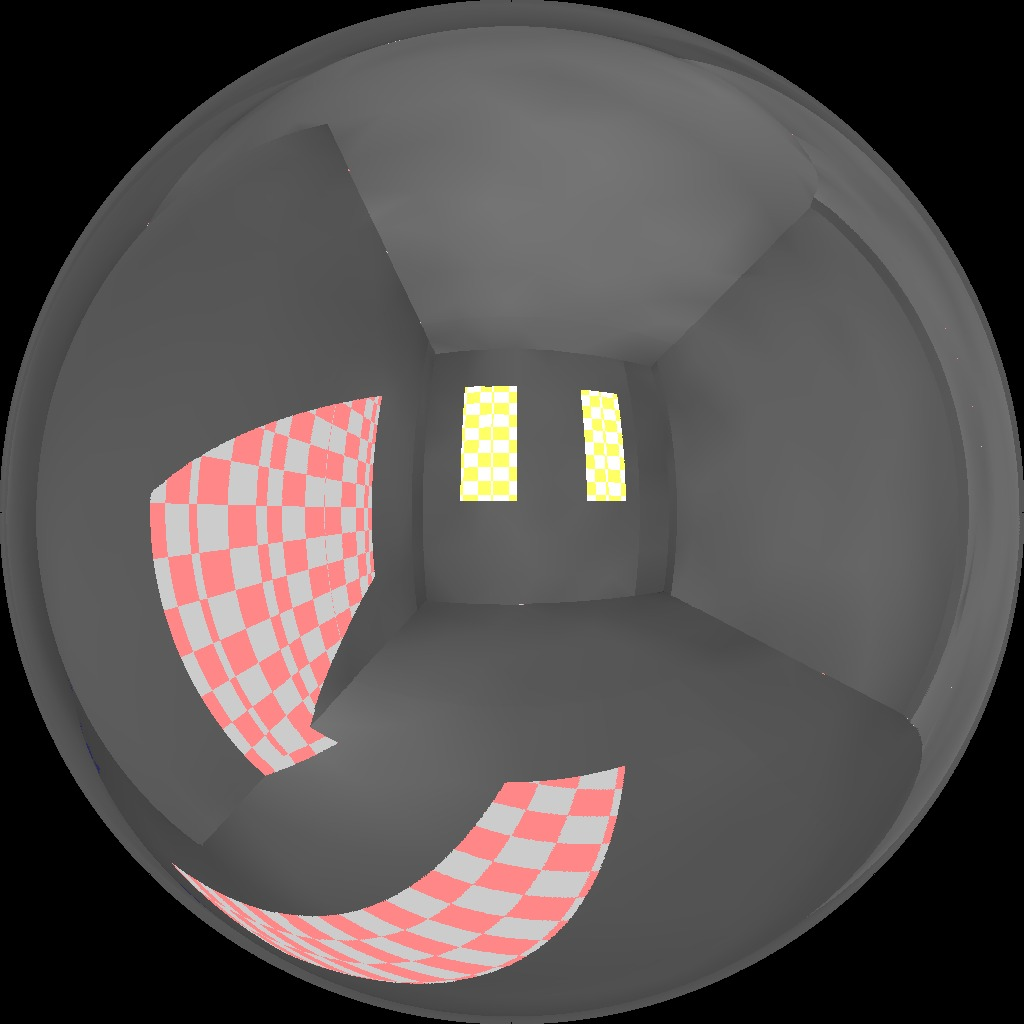
\includegraphics{wallfiles/mrc331/surface_camera_VIEW_person3.jpg}}
\resizebox{\picwidth}{!}{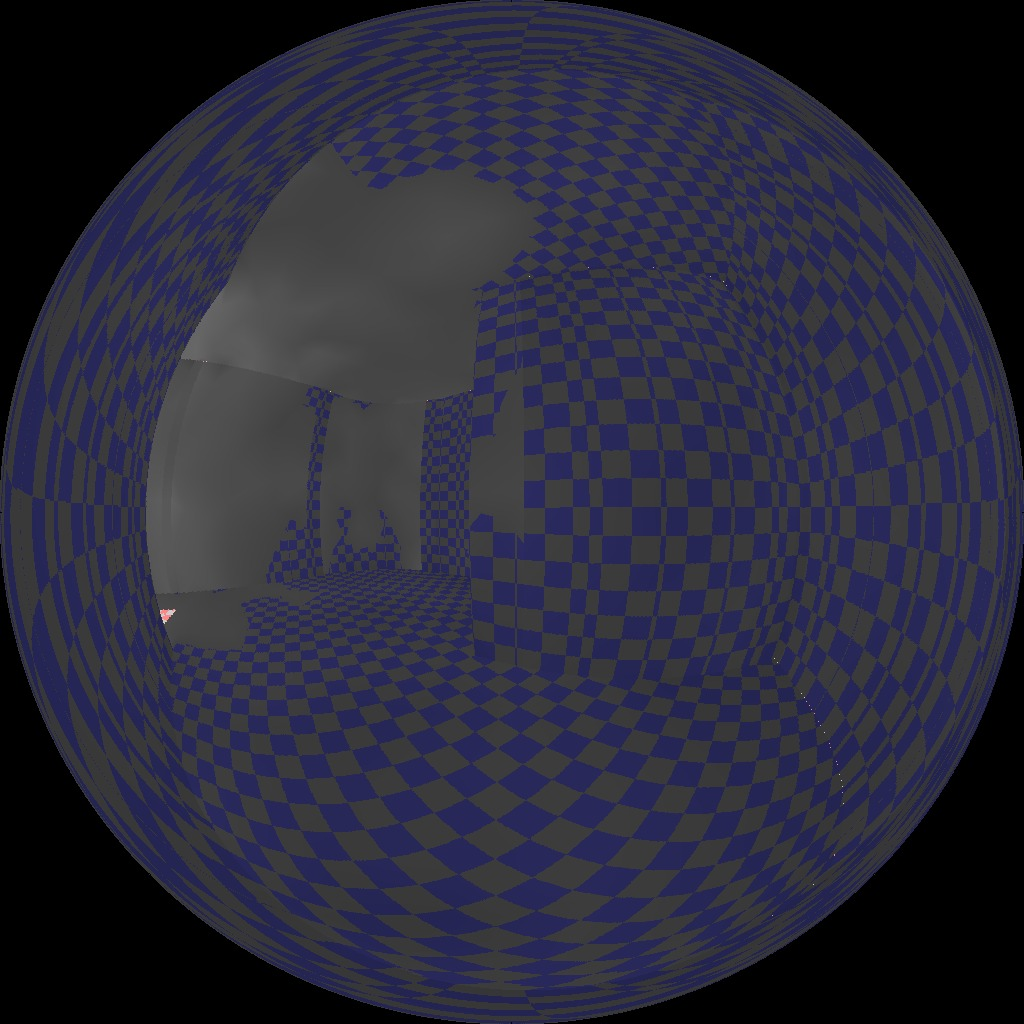
\includegraphics{wallfiles/mrc331/surface_camera_VIEW_person4.jpg}}
\resizebox{\picwidth}{!}{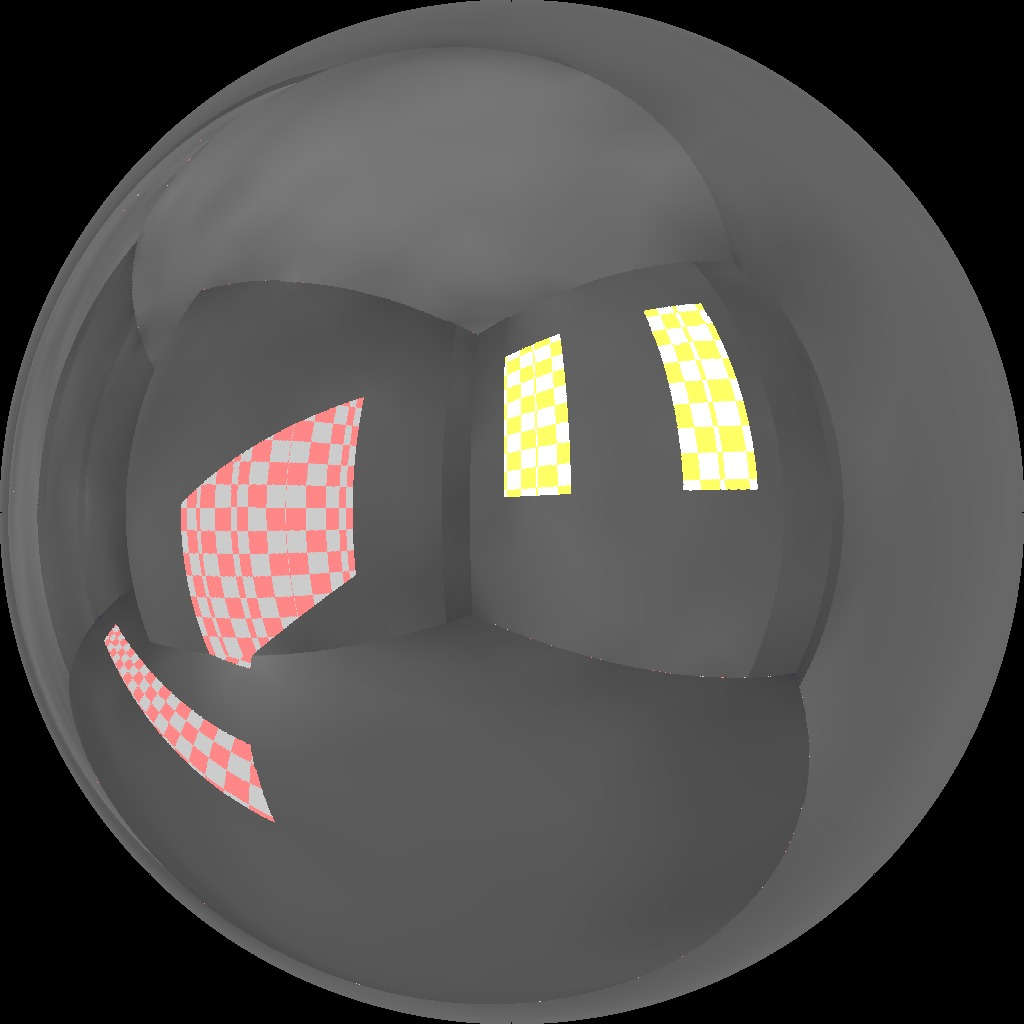
\includegraphics{wallfiles/mrc331/surface_camera_VIEW_person5.jpg}}
\caption{Fisheye views were provided at the position and view
  direction of each glare avatar to allow the users to experience the
  lighting problems from the perspective of inside the office model shown in Figure~\ref{FIGURE:office_false_color}.
  Illumination problems can vary significantly across different
  perspectives within the same space.}
\vspace{-0.15in}
\label{FIGURE:fisheyes}
\end{figure*}

\subsection{Photon mapping}







\begin{figure*}[t]
\begin{center}
\newcommand{\picheight}{2.5in}
%\resizebox{\picheight}{!}{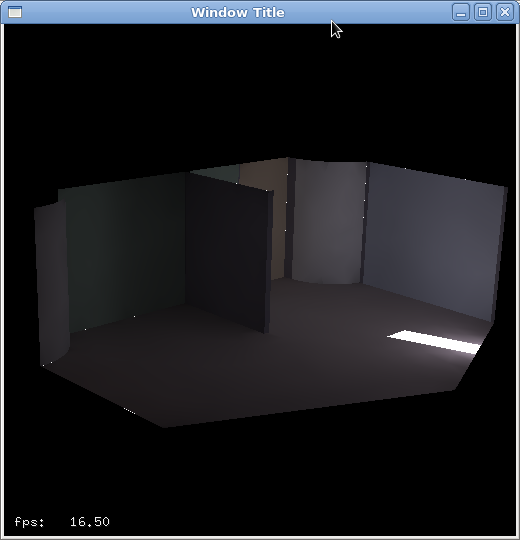
\includegraphics{wallfiles/cool_floor/cool_floor_normal_render.png}}
%\resizebox{\picheight}{!}{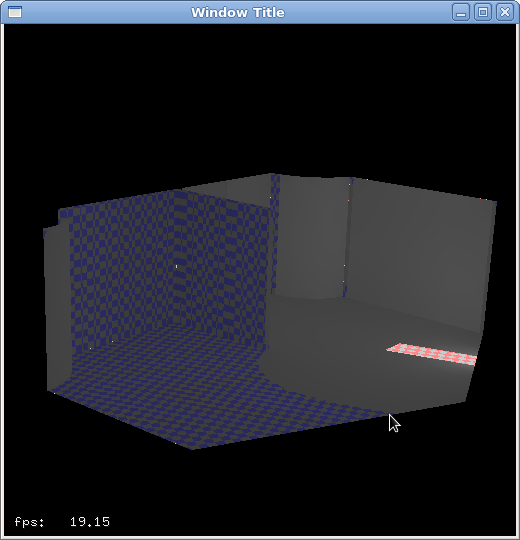
\includegraphics{wallfiles/cool_floor/cool_floor_false_color.png}}
\resizebox{!}{\picheight}{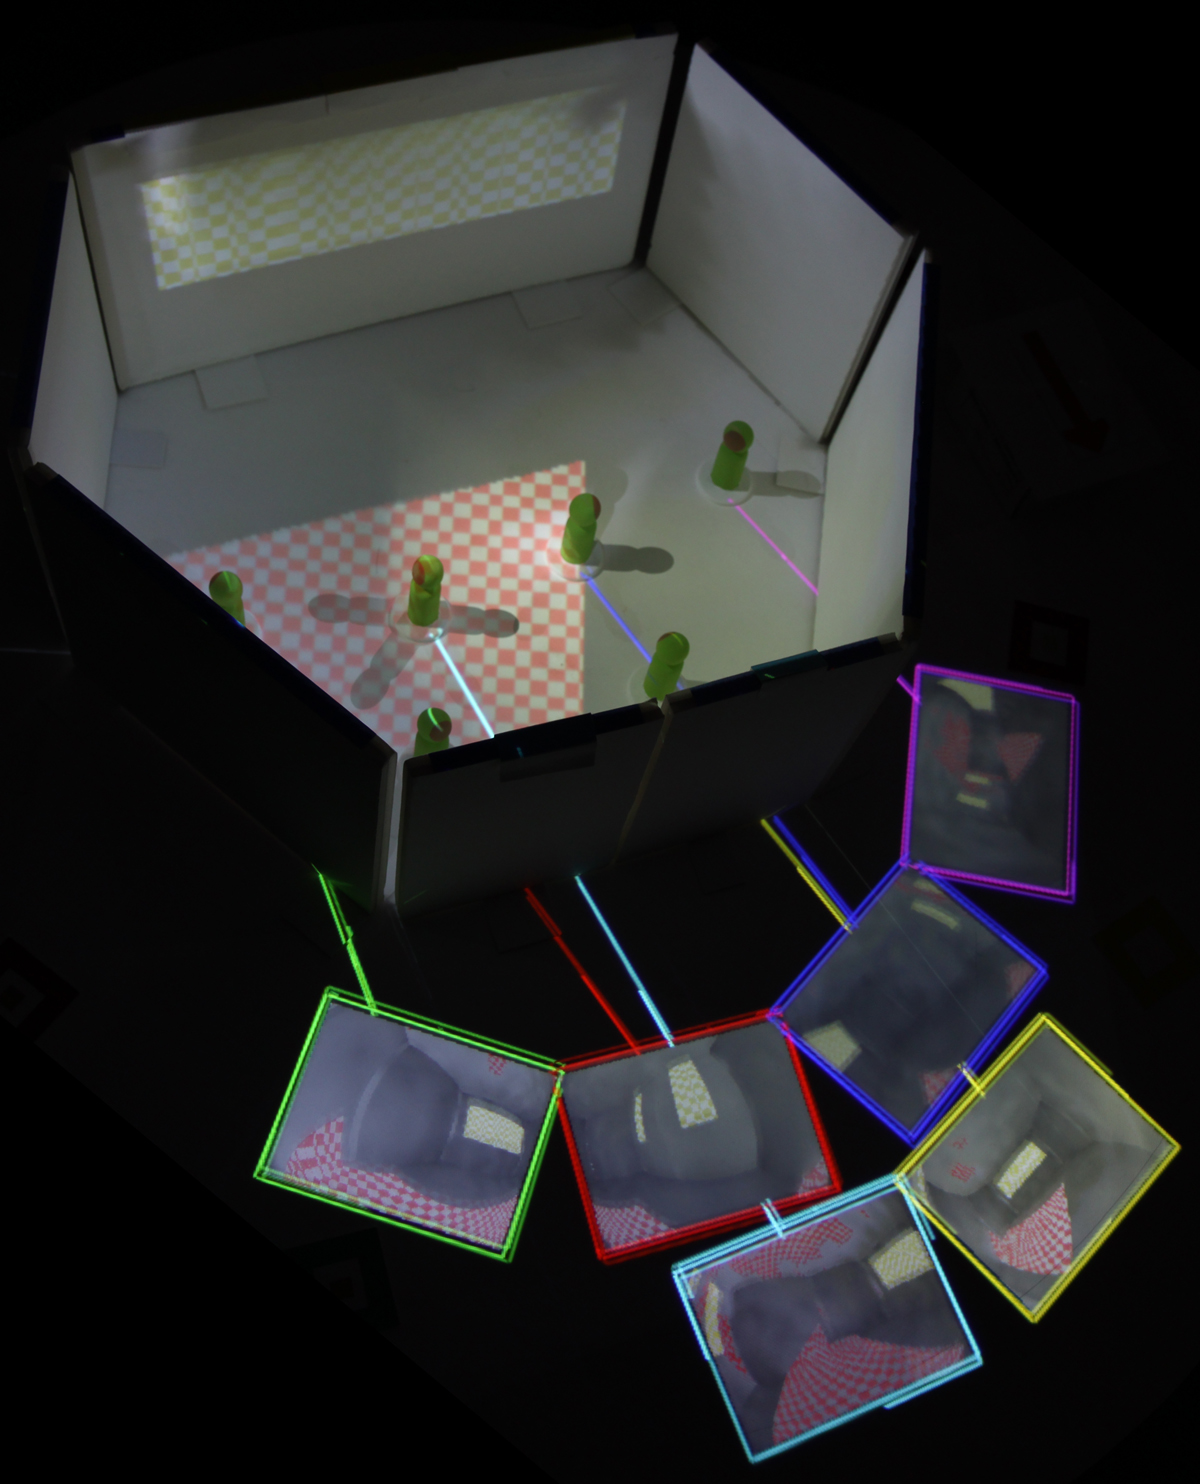
\includegraphics{photos/museum_false_color_nocurved.jpg}}
%\resizebox{\picheight}{!}{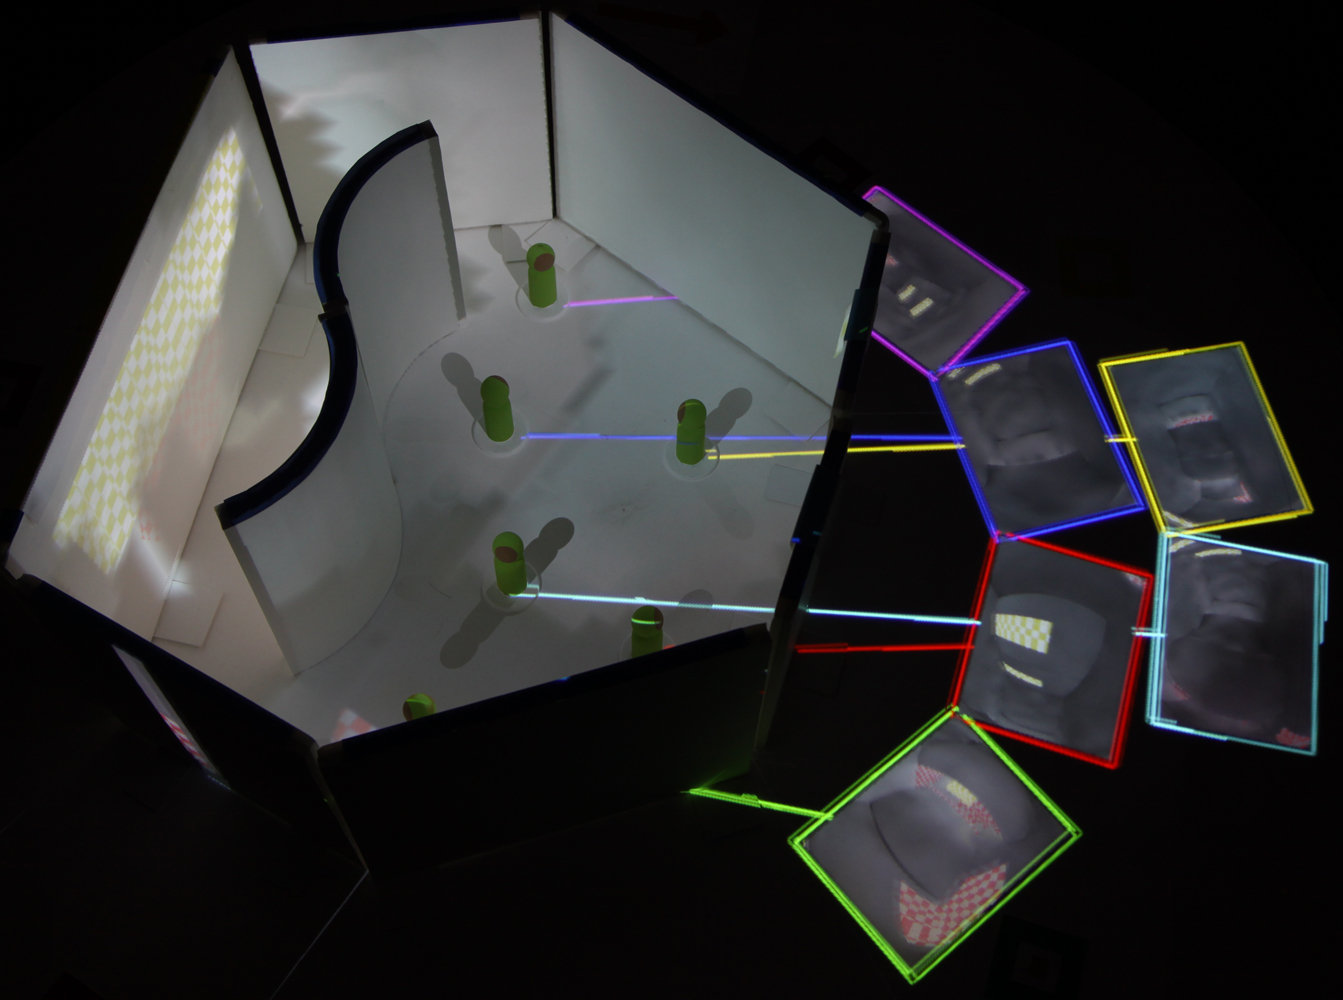
\includegraphics{photos/museum_false_color_curved.jpg}}
\resizebox{!}{\picheight}{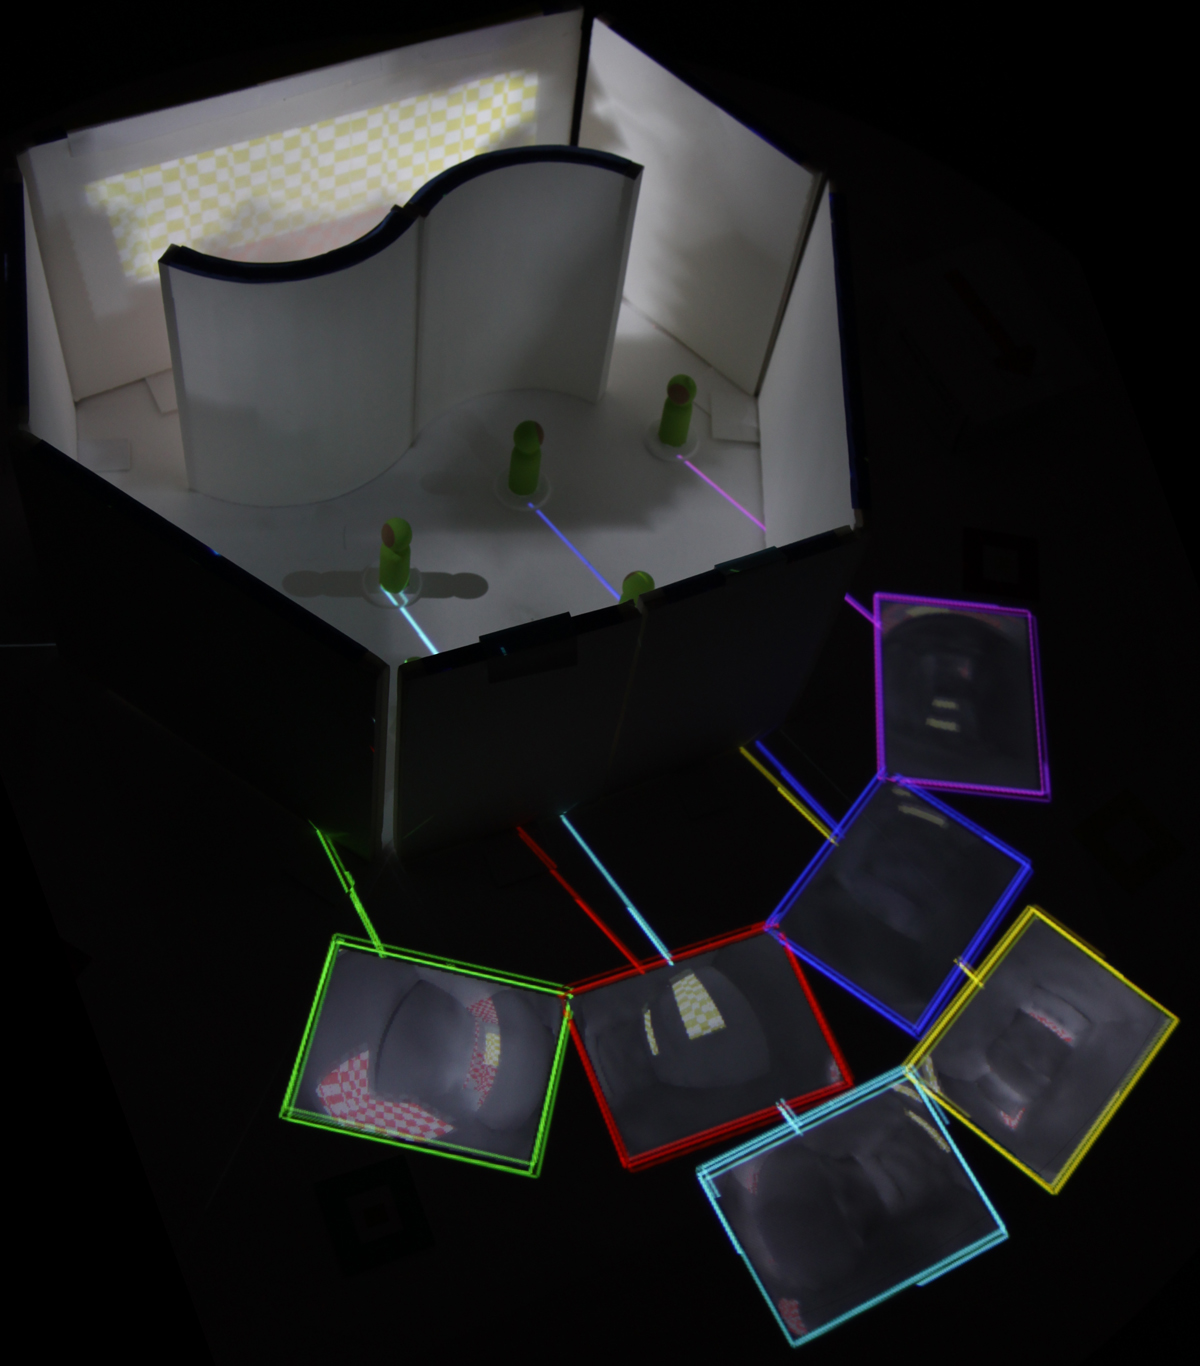
\includegraphics{photos/museum_false_color2.jpg}}
\vspace{-0.1in}
\end{center}
\caption{ On the left is a potential design for an art gallery.  The
  rendering in the room and the glare views both show significant
  over-illumination and glare problems.  On the right is a potential
  renovation to reduce glare. The renderings of the room from each
  avatar are shown in Figure~\ref{FIGURE:museum2}.}
%
%The most common problem users encountered in our user study
%  was determining the areas that were too bright or too dark.  Our
%  false color visualizations will help future user discern where the
%  problem areas are.  The blue checkerboard is the under-illuminated
%  area and the red checkerboard is the over-illuminated area.
%
%}
%\vspace{-0.15in}
%\label{FIGURE:cool_floor}
\label{FIGURE:editing_model}
\end{figure*}





\begin{figure*}[t]
\newcommand{\picwidth}{.95in}
\resizebox{\picwidth}{!}{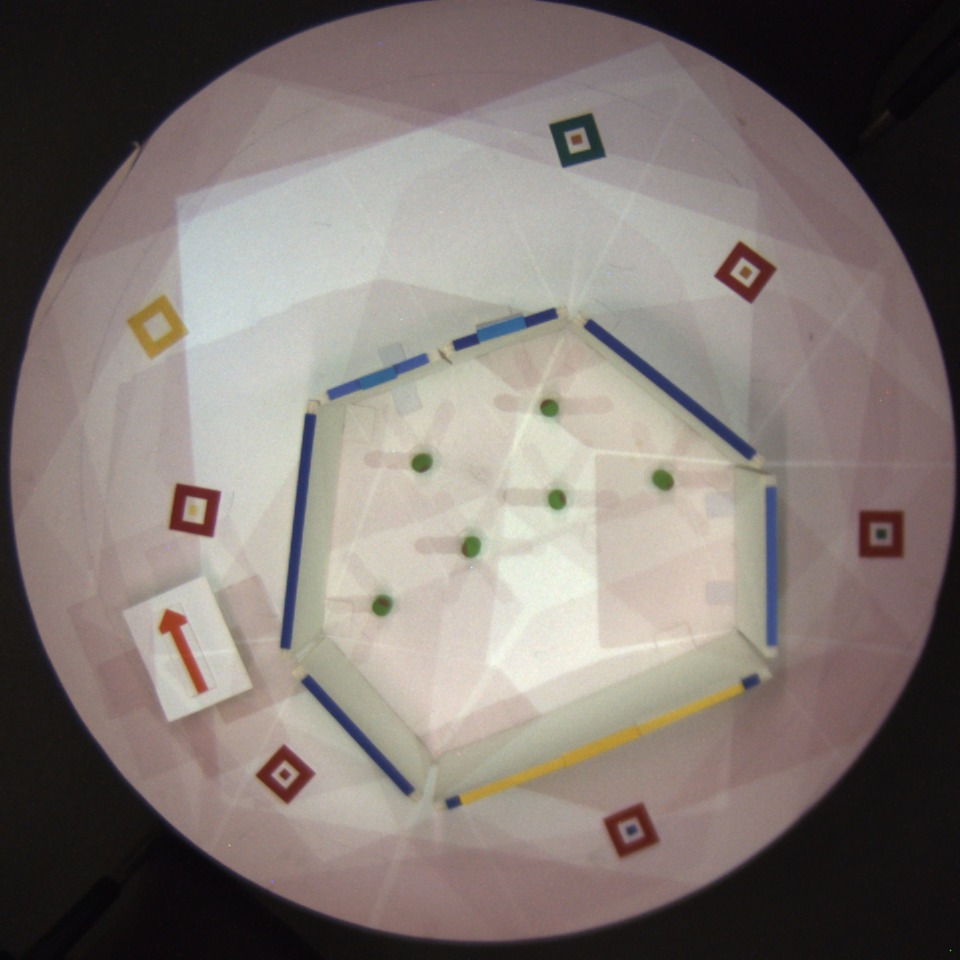
\includegraphics{wallfiles/museum2_false_nocurved/out.jpg}}
\resizebox{\picwidth}{!}{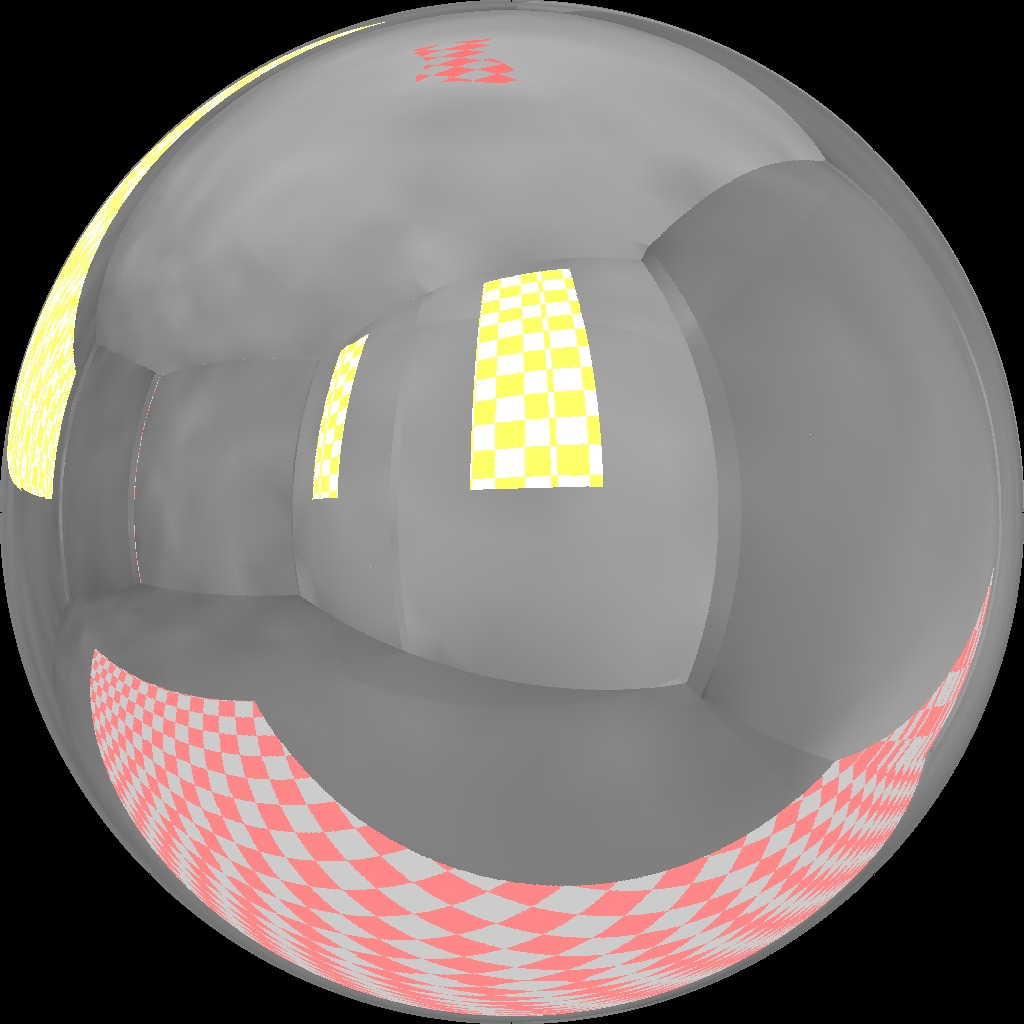
\includegraphics{wallfiles/museum2_false_nocurved/surface_camera_VIEW_person0.jpg}}
\resizebox{\picwidth}{!}{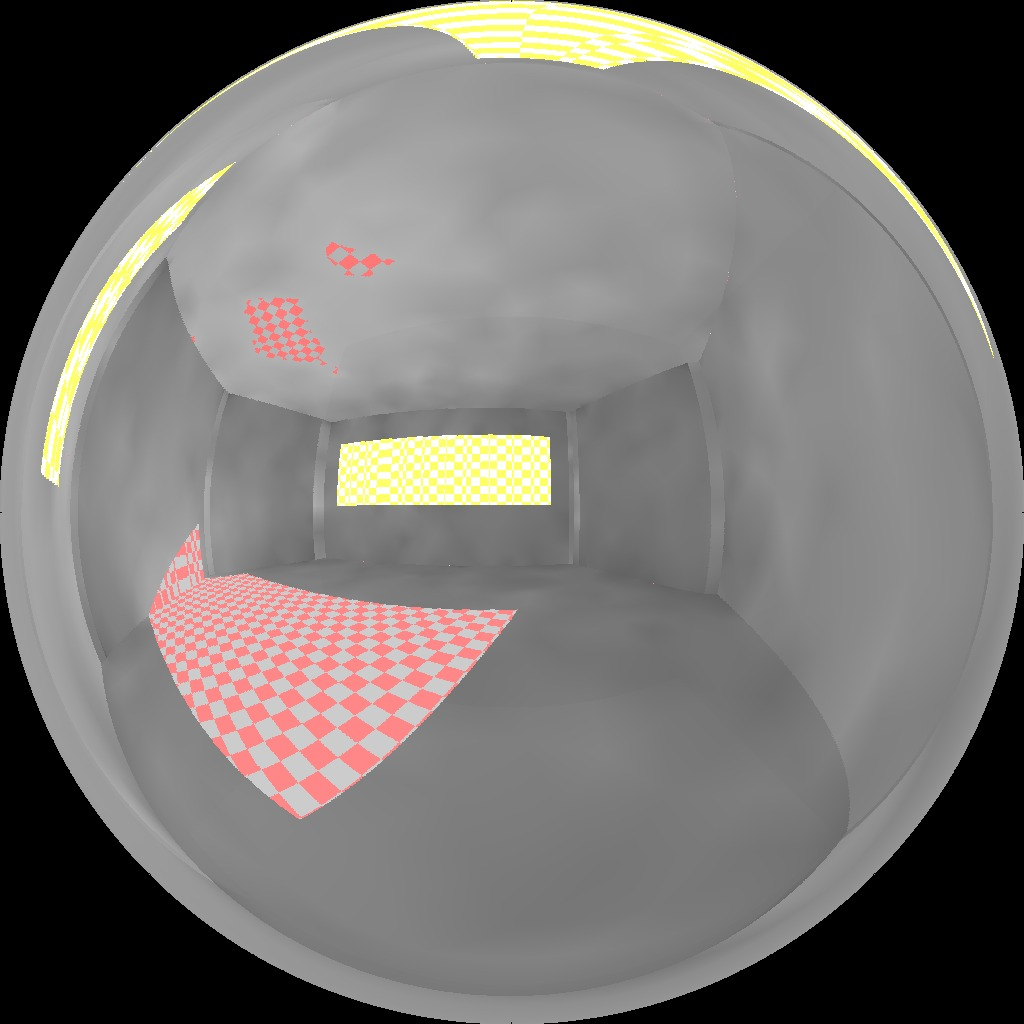
\includegraphics{wallfiles/museum2_false_nocurved/surface_camera_VIEW_person1.jpg}}
\resizebox{\picwidth}{!}{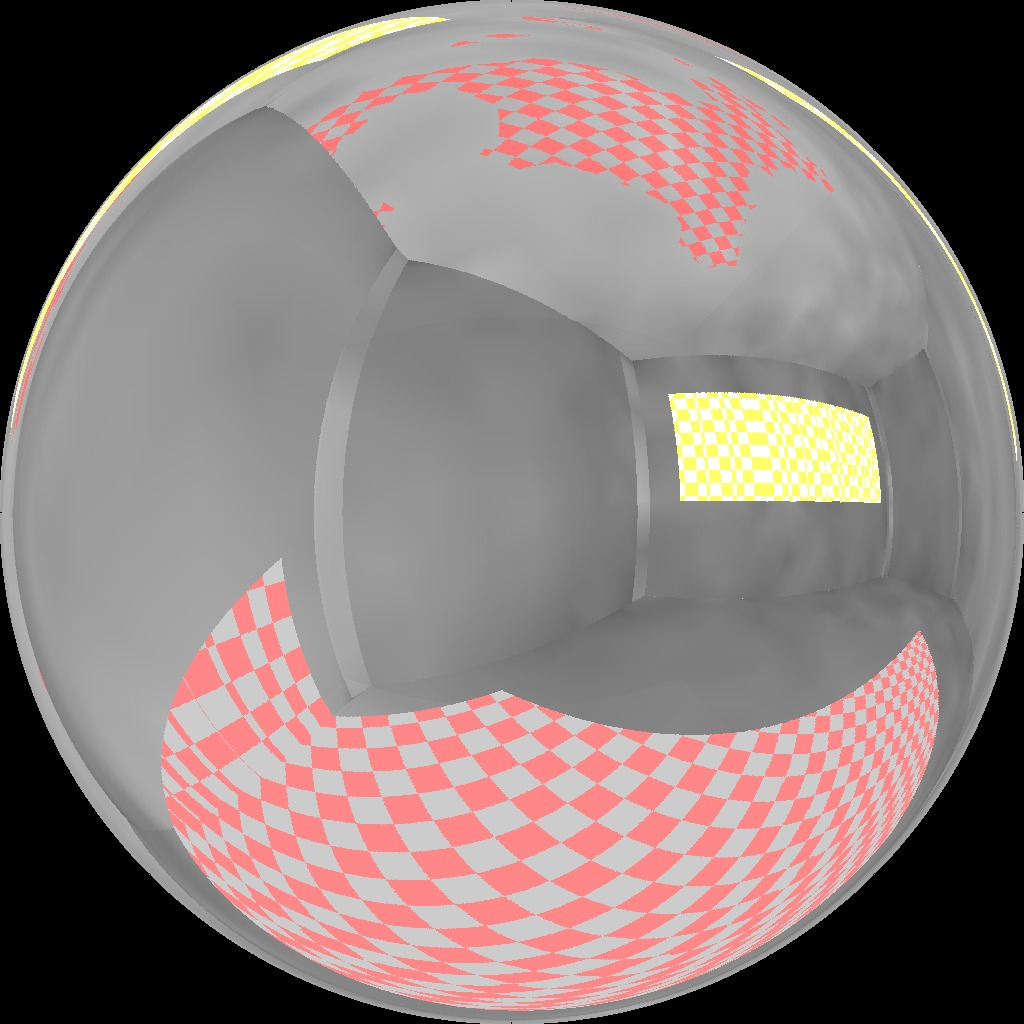
\includegraphics{wallfiles/museum2_false_nocurved/surface_camera_VIEW_person2.jpg}}
\resizebox{\picwidth}{!}{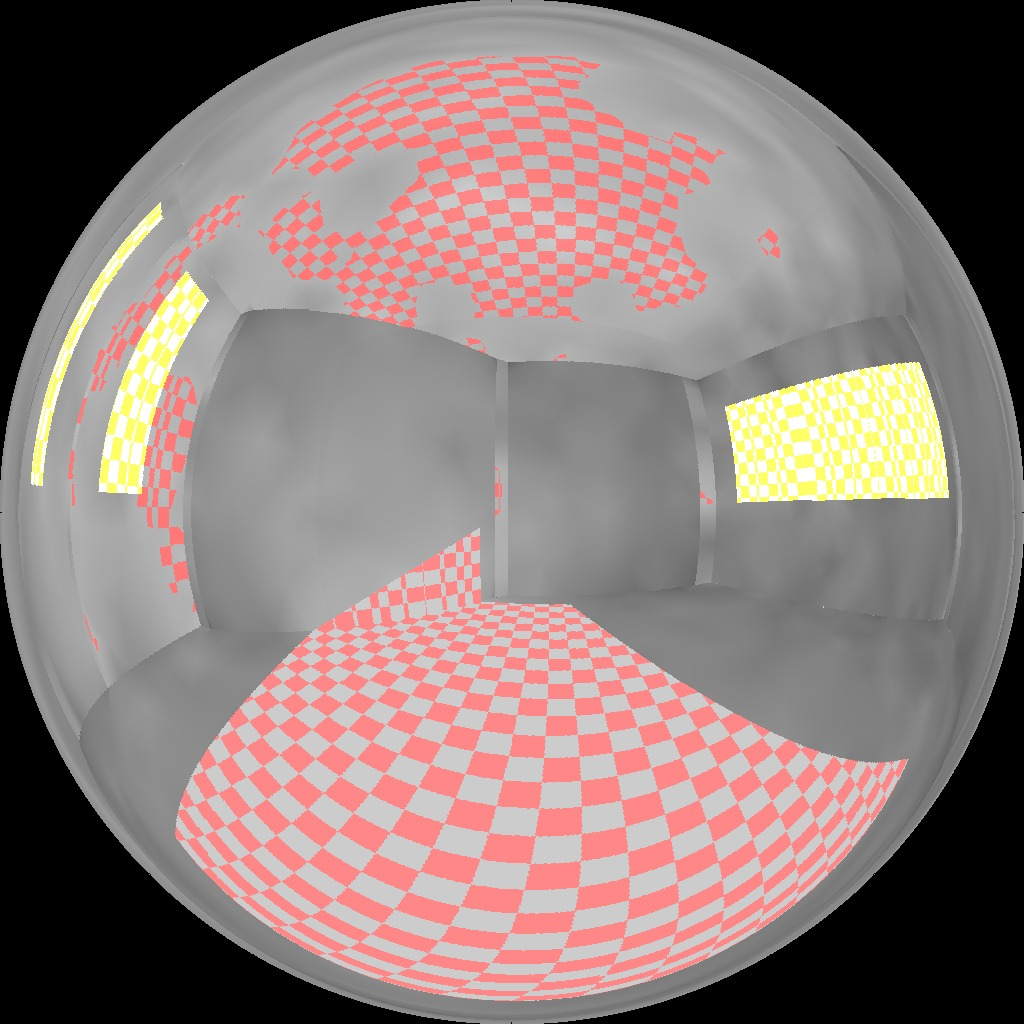
\includegraphics{wallfiles/museum2_false_nocurved/surface_camera_VIEW_person3.jpg}}
\resizebox{\picwidth}{!}{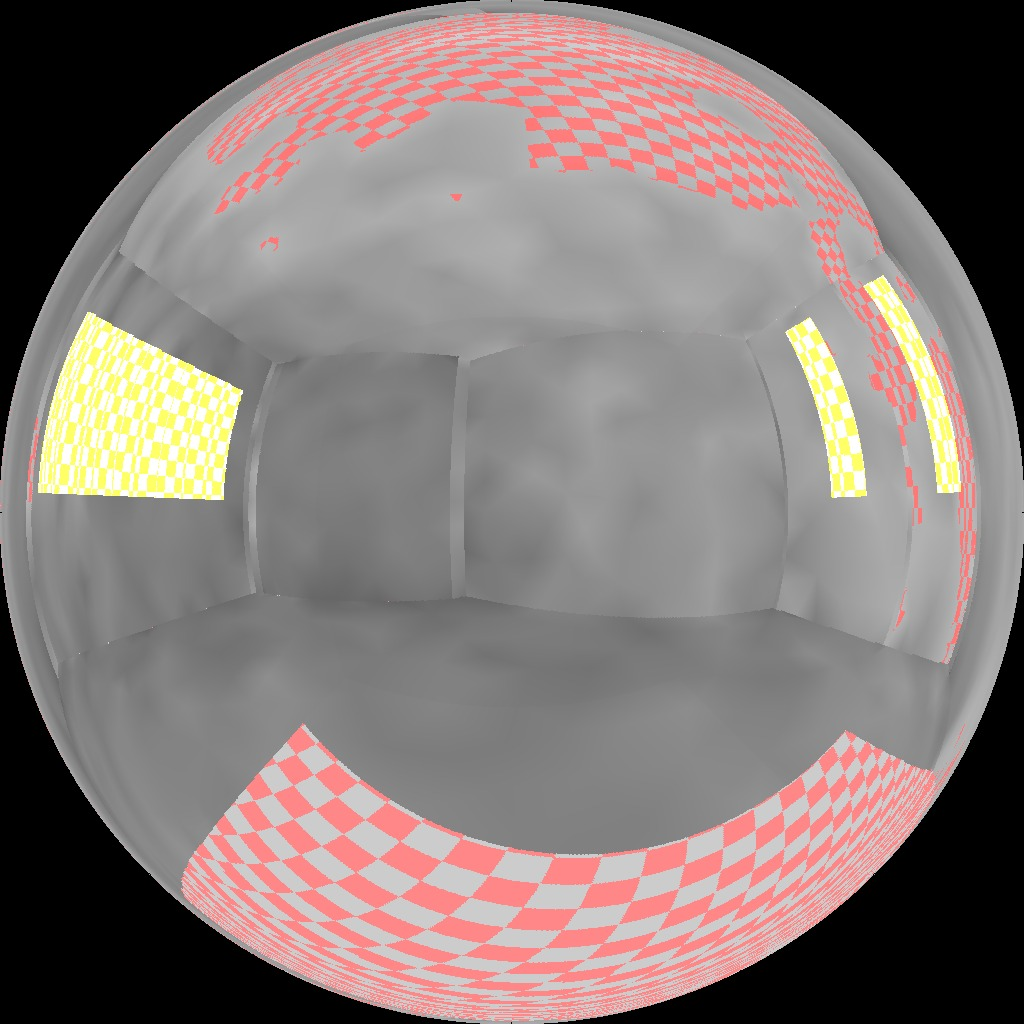
\includegraphics{wallfiles/museum2_false_nocurved/surface_camera_VIEW_person4.jpg}}
\resizebox{\picwidth}{!}{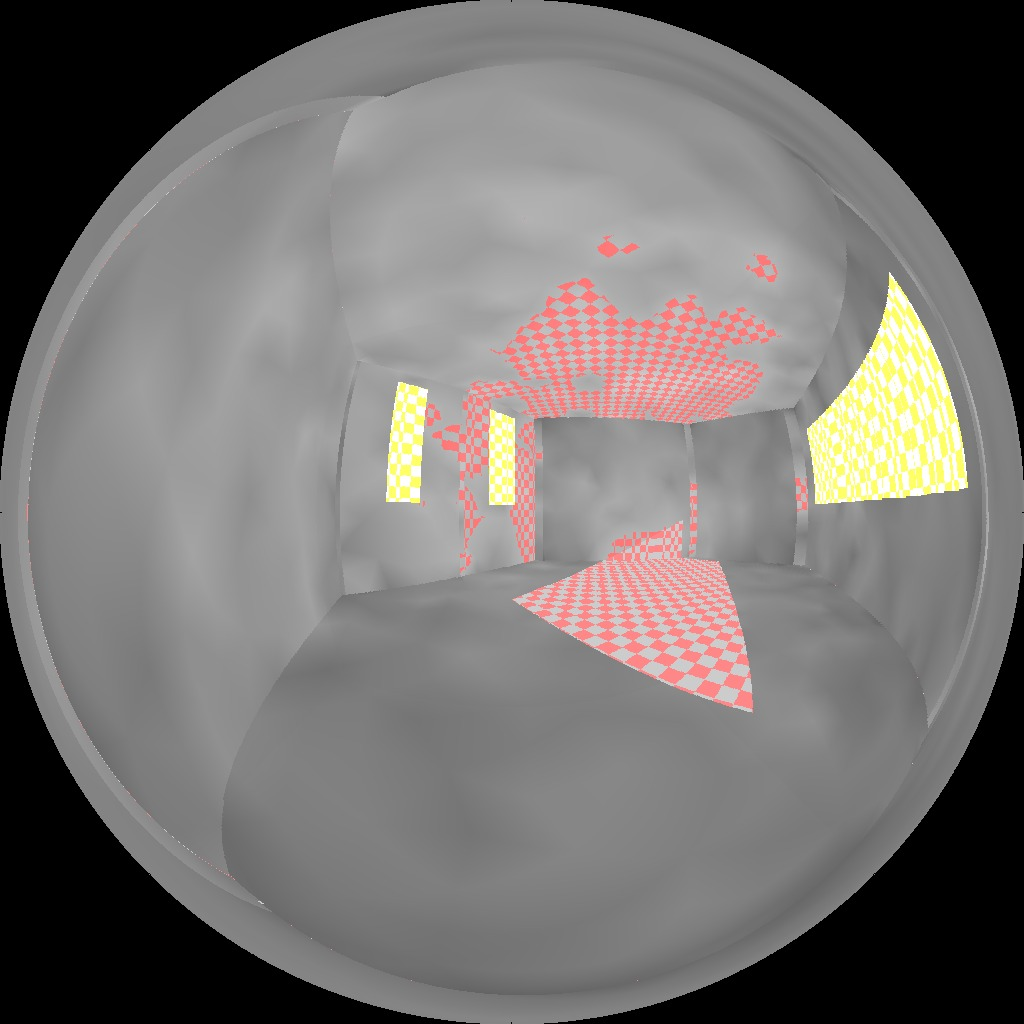
\includegraphics{wallfiles/museum2_false_nocurved/surface_camera_VIEW_person5.jpg}}
\\
\resizebox{\picwidth}{!}{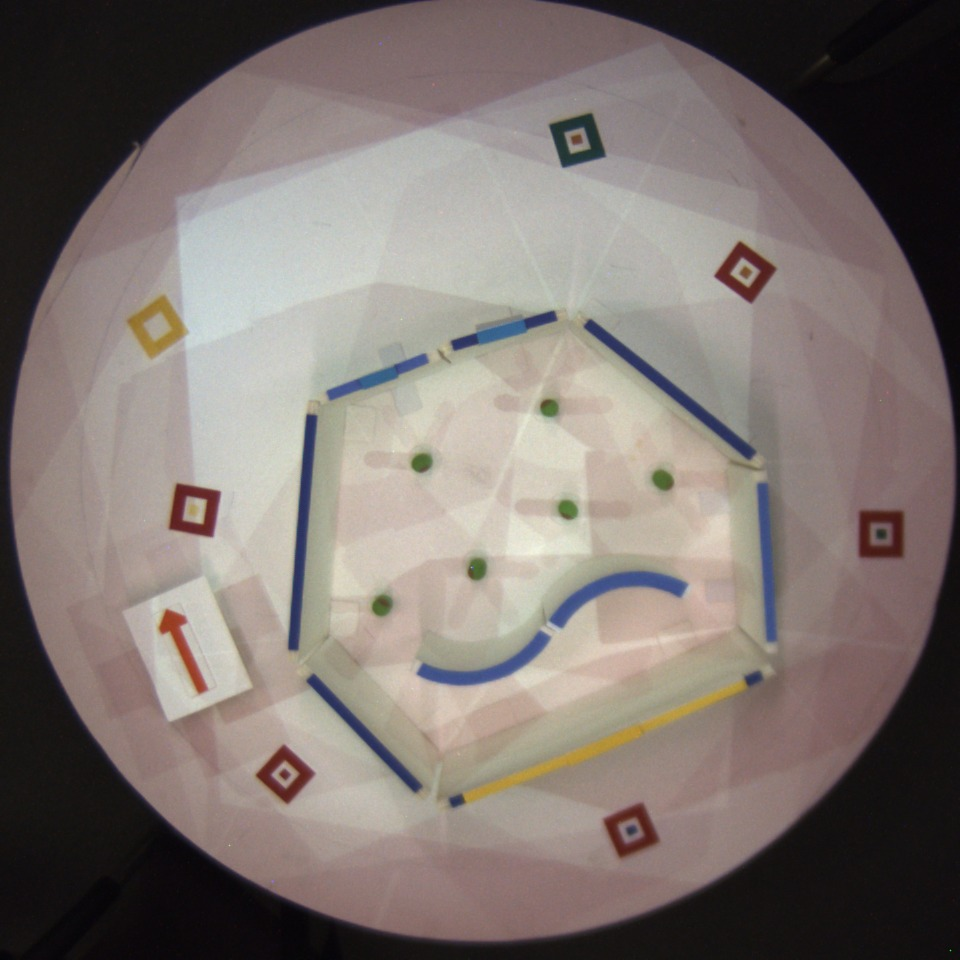
\includegraphics{wallfiles/museum2_false/out.jpg}}
\resizebox{\picwidth}{!}{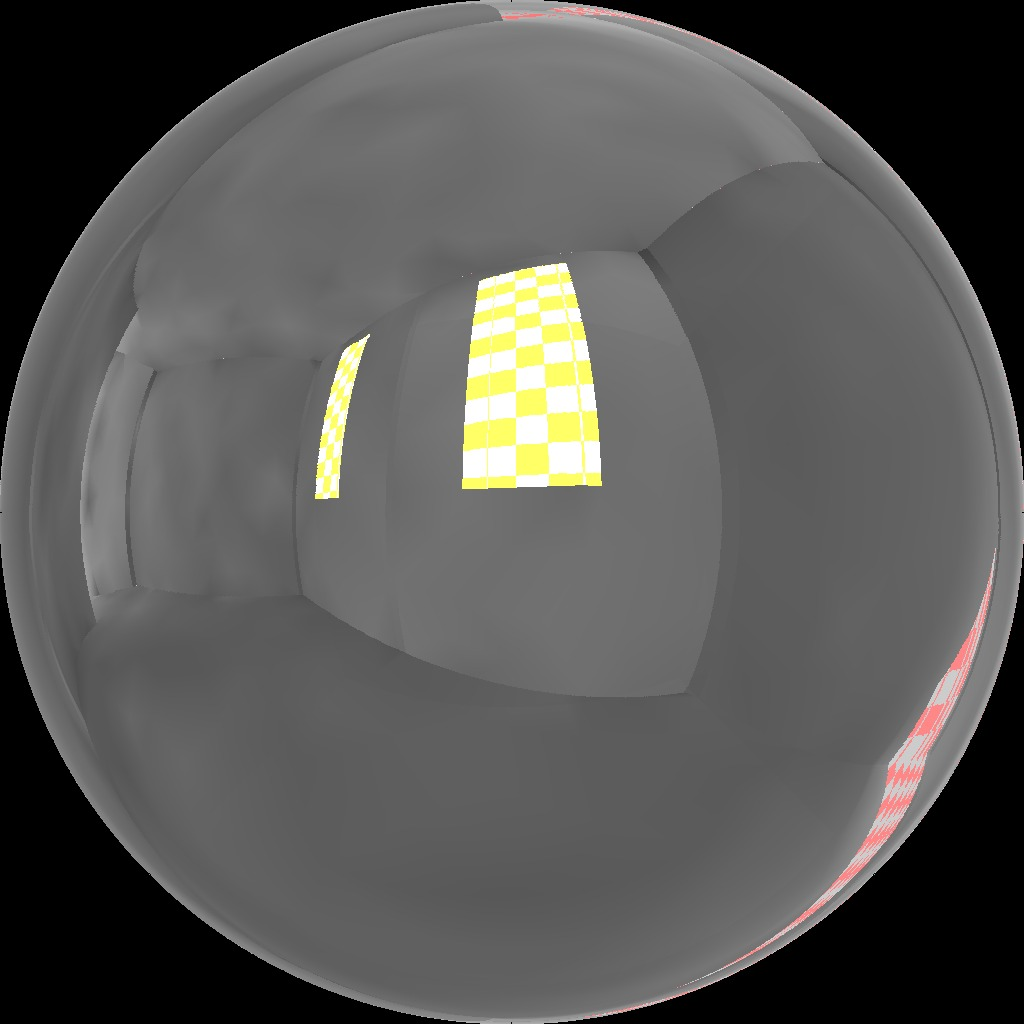
\includegraphics{wallfiles/museum2_false/surface_camera_VIEW_person0.jpg}}
\resizebox{\picwidth}{!}{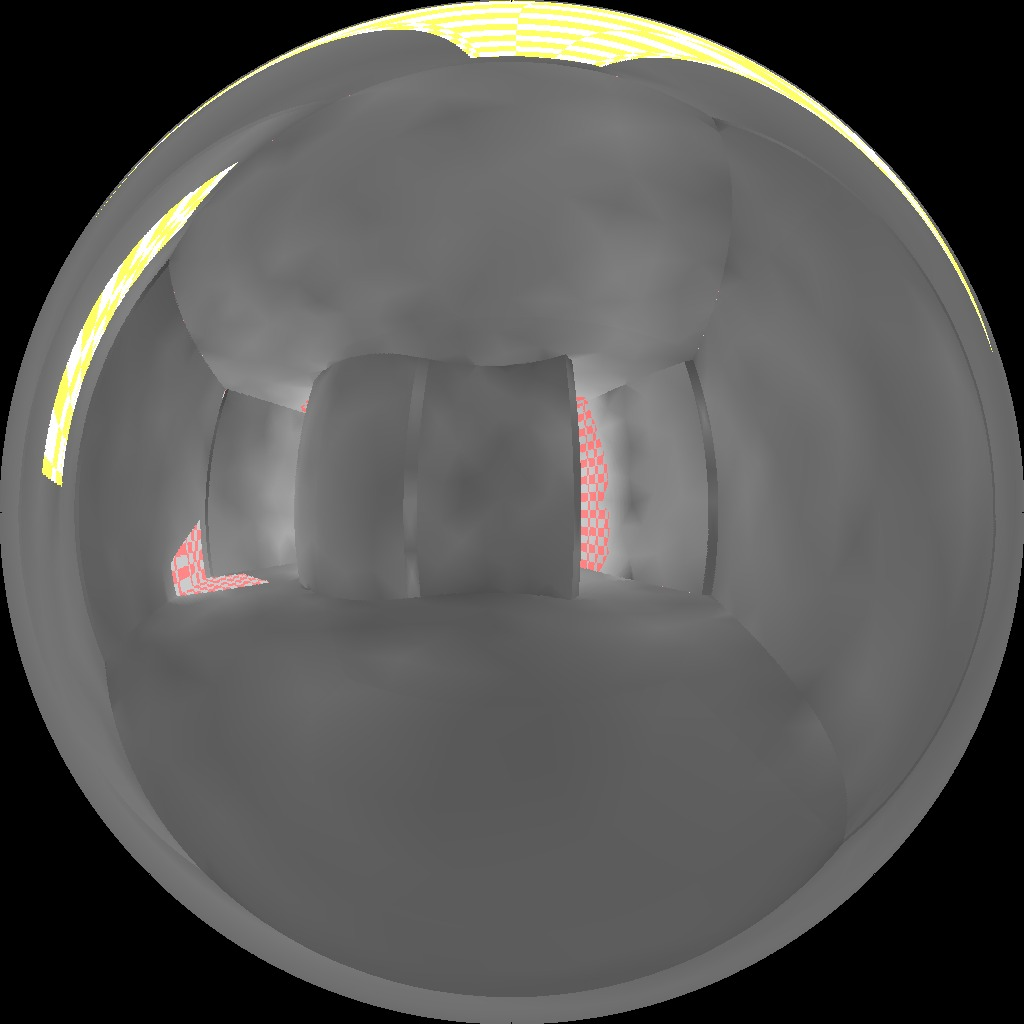
\includegraphics{wallfiles/museum2_false/surface_camera_VIEW_person1.jpg}}
\resizebox{\picwidth}{!}{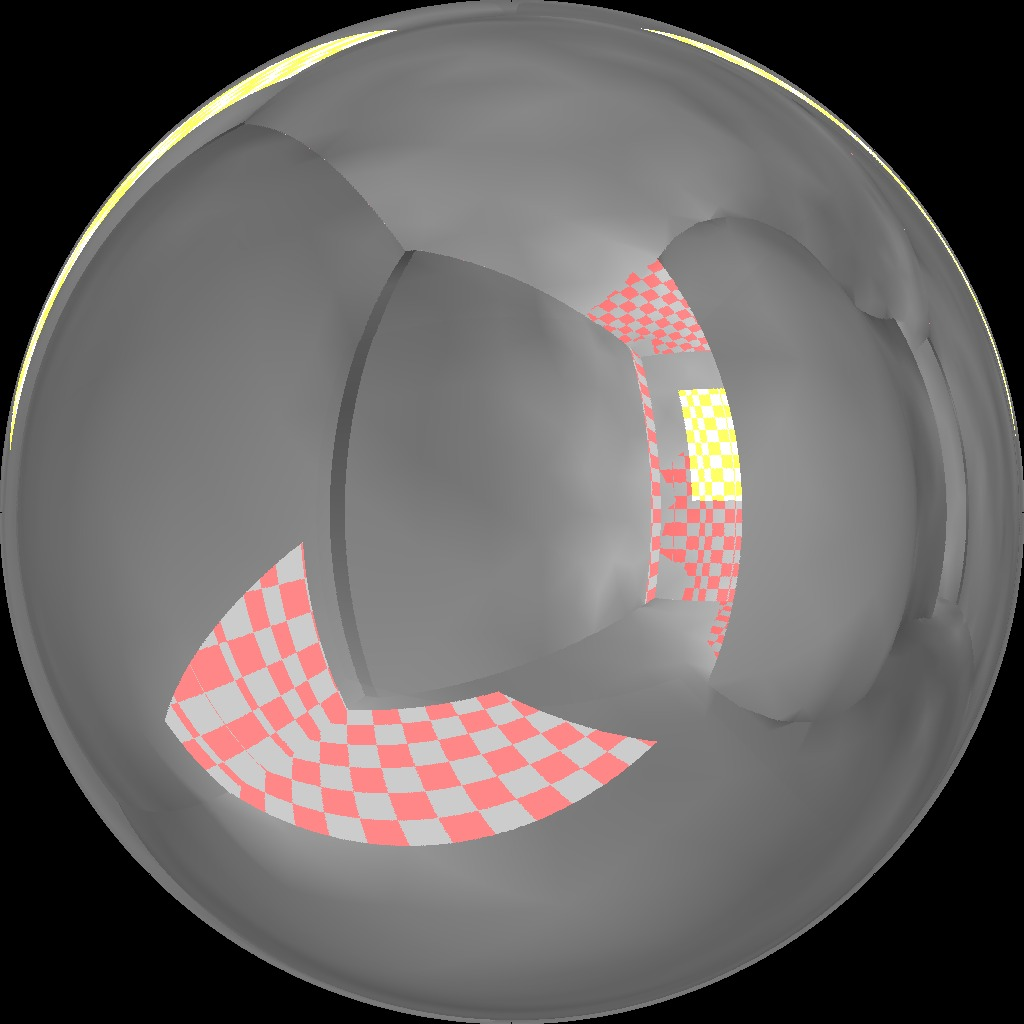
\includegraphics{wallfiles/museum2_false/surface_camera_VIEW_person2.jpg}}
\resizebox{\picwidth}{!}{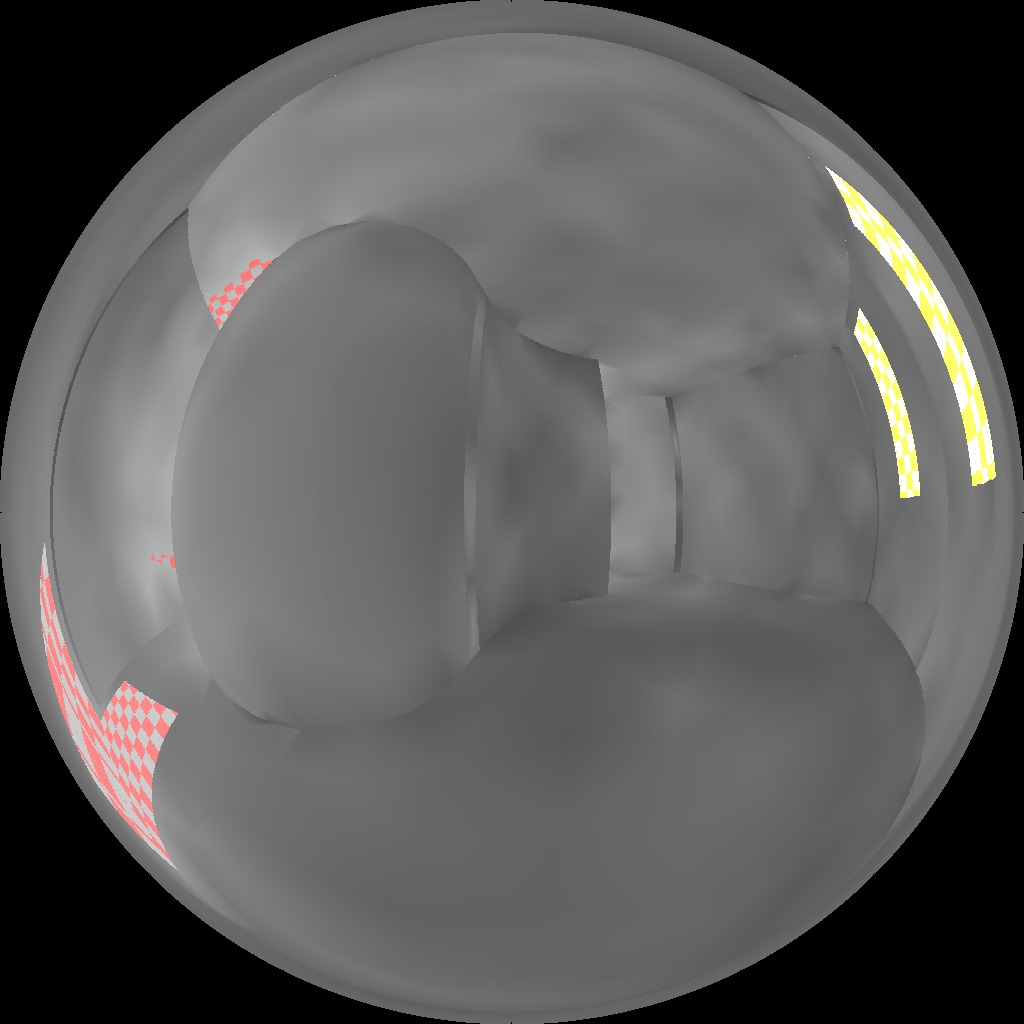
\includegraphics{wallfiles/museum2_false/surface_camera_VIEW_person3.jpg}}
\resizebox{\picwidth}{!}{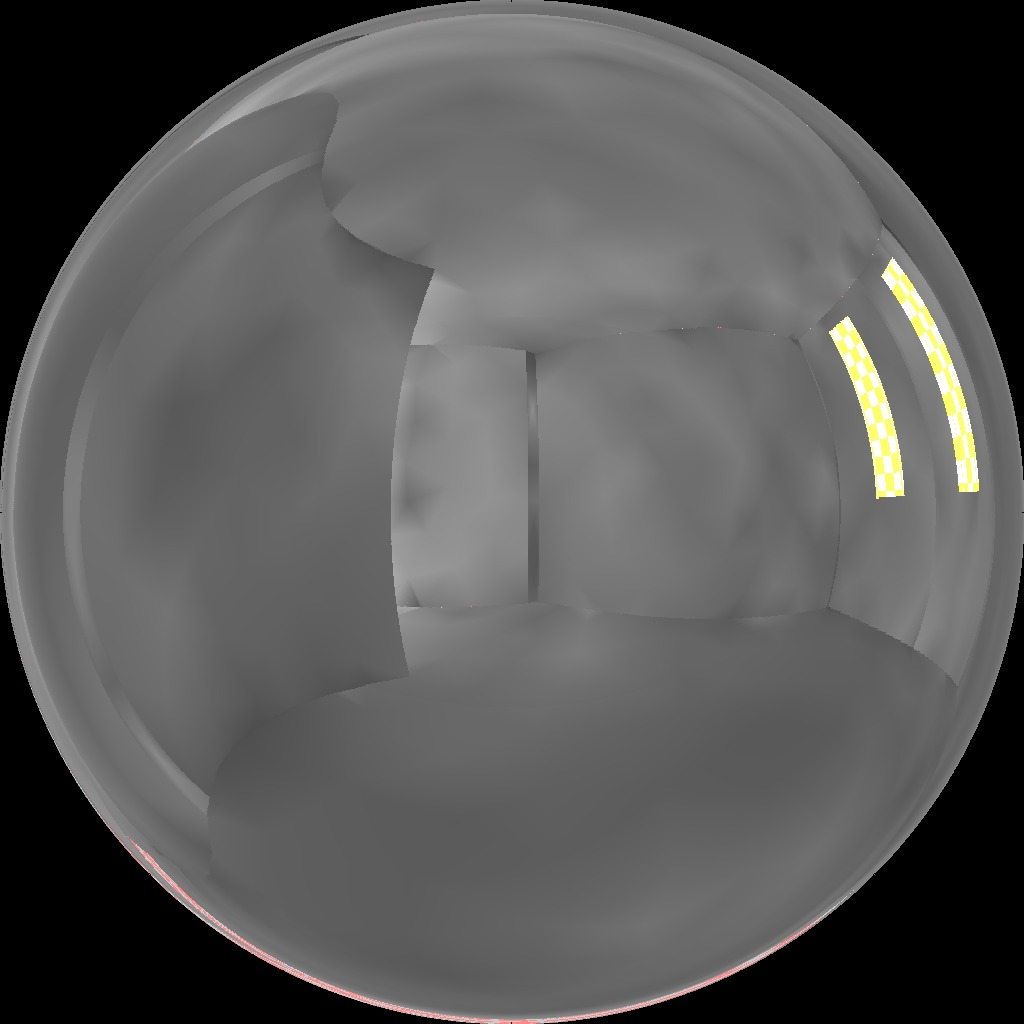
\includegraphics{wallfiles/museum2_false/surface_camera_VIEW_person4.jpg}}
\resizebox{\picwidth}{!}{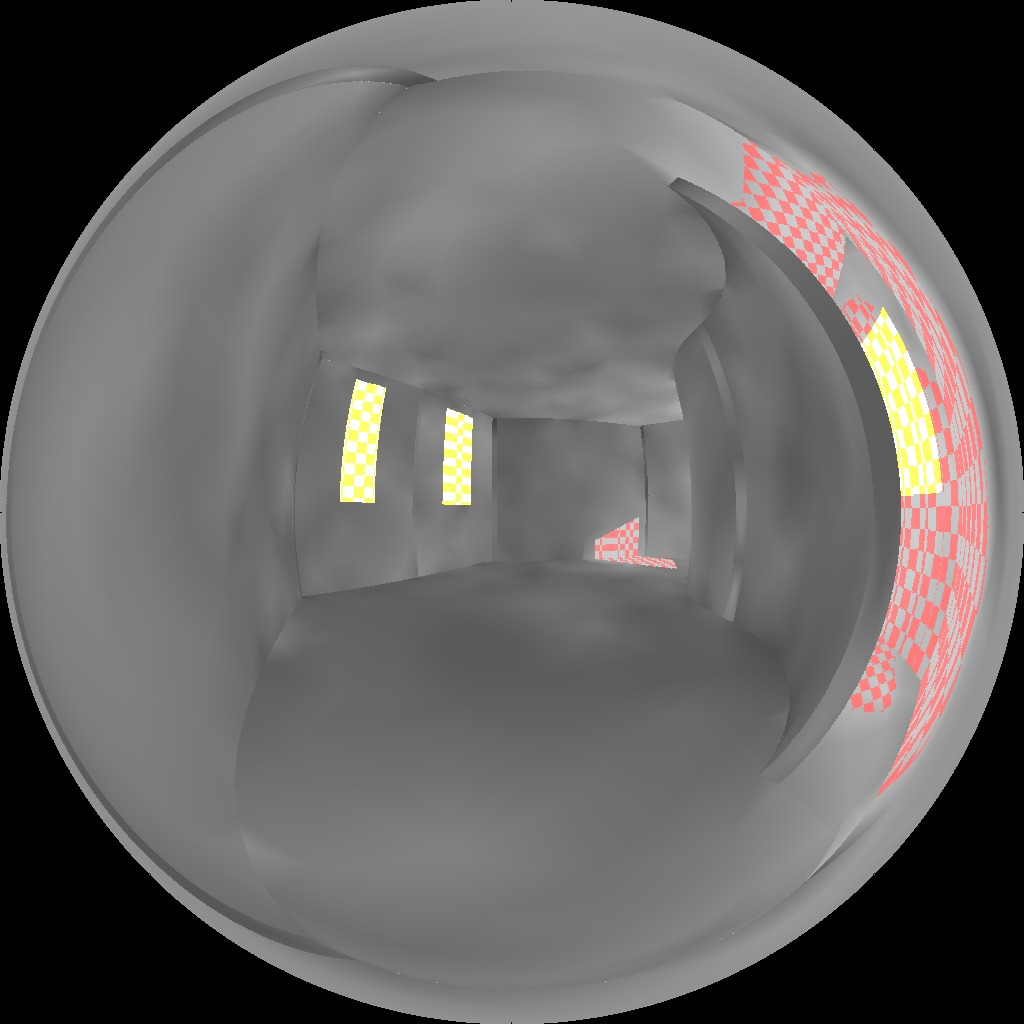
\includegraphics{wallfiles/museum2_false/surface_camera_VIEW_person5.jpg}}

%\vspace{-0.1in}
\caption{This museum space model from Figure~\ref{FIGURE:editing_model} had
  significant glare problems.  By adding a curved wall in the middle,
  the glare problems are significantly reduced.}
\vspace{-0.15in}
\label{FIGURE:museum2}
\end{figure*}


\subsection{Photon mapping}

In the rendering method used in our system, light is simulated
bouncing through the scene through the use of \emph{photons}.  Photon
Mapping is a method where photons are sent from a light source,
allowed to bounce around a scene and then gathered at specific
locations throughout the scene in order to be
rendered\cite{Jensen:1996:GIU:275458.275461}.  Image space photon
mapping was a GPU-accelerated version of photon mapping which allowed
interactive rendering time \cite{mcguire09imagespace}.  Our renderer
is based on an extension of this photon mapper which began
investigating how to use the sun and sky as a light source for image
spaced photon mapping \cite{ericli}.



\section{Motivation and Current Work}

Rendering has traditionally been a field where generating an
aesthetically pleasing image has been a higher priority than physical
accuracy.  In architectural design, physical accuracy is just as
important as the appearance of the rendering.  Knowing the locations
suffering from over-illumination, under-illumination, and glare directly
impacts how useful a space is to potential occupants.  In spaces like
art galleries, this is particularly relevant as direct sunlight can
damage artwork. 
In a classroom, proper illumination is important both so that students can 
read the chalkboard, books and laptops and so that the teacher and students 
can communicate well.
Office environments need proper lighting because workers spend 40-60 hours 
in them per week and employers want to minimize fatigue and discomfort.
While accuracy is important to creating a usable and comfortable space, 
it is not sufficient to create an
effective renderer.  Architectural daylighting design is both the
process of admitting and redirecting an appropriate amount of light
and making creating aesthetic choices to create comfortable,
beautiful, and interesting spaces that offer healthy, productive, and
inspiring work and play environments.  We have also incorporated the
simulation of intricate screens to the windows to illustrate one way
our interface allows architects to make these choices.


%Rendering has traditionally been a field where generating an
%aesthetically pleasing image has been a higher priority than physical
%accuracy.  In architectural design, physical accuracy is just as
%important as the appearance of the rendering.  Knowing the locations
%suffering from overillumination, underillumination and glare directly
%impacts how useful a space is to potential occupants.  In spaces like
%art gallaries, this is particularly relevant as direct sunlight can
%damage artwork.  While accuracy is important, it is not sufficient to
%create an effective renderer.  Architectural daylighting is both the
%process of choosing an appropriate amount of light and making creative
%aesthetic choices.  We chose to add intricate screens to the windows
%to illustrate one way our interface allows architects to make these
%choices.


\begin{figure*}[t]
\newcommand{\picwidth}{1.68in}
\resizebox{\picwidth}{!}{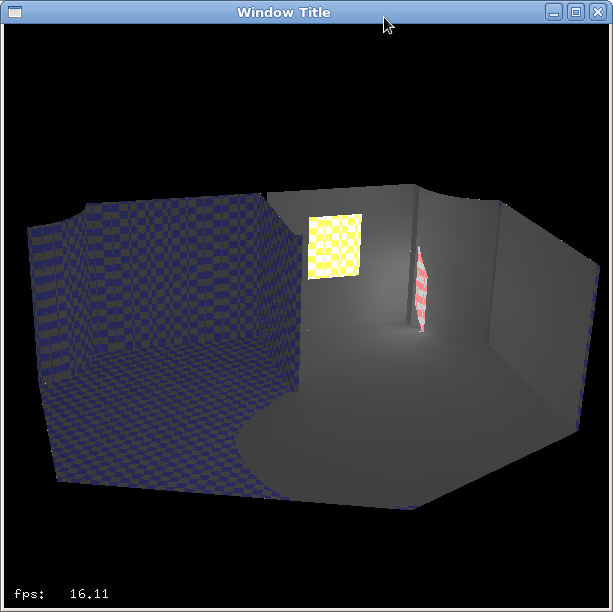
\includegraphics{wallfiles/mrc331/mrc331_6_21_7am.png}}
\resizebox{\picwidth}{!}{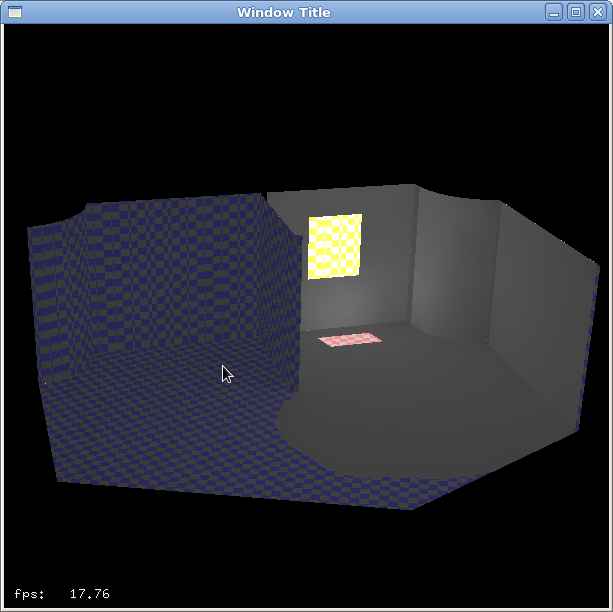
\includegraphics{wallfiles/mrc331/mrc331_6_21_11am.png}}
\resizebox{\picwidth}{!}{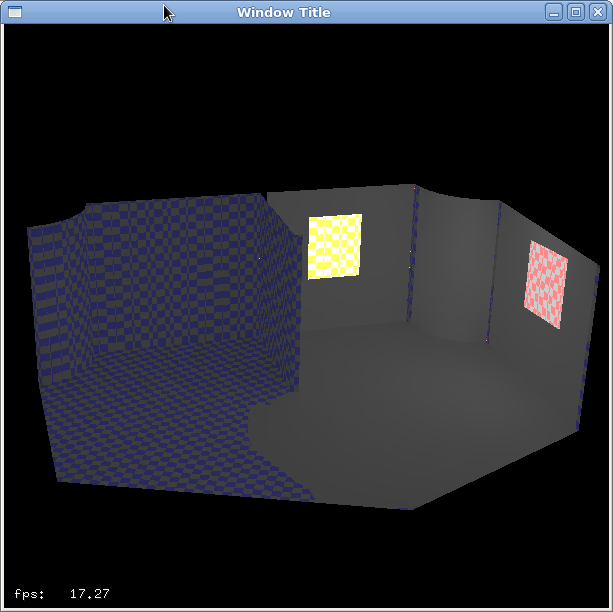
\includegraphics{wallfiles/mrc331/mrc331_12_21_7am.png}}
\resizebox{\picwidth}{!}{\includegraphics{wallfiles/mrc331/mrc331_12_21_11am.png}}%
%\vspace{-0.1in}
\caption{Over-illumination and Under-illumination are drastically
  different at different times and dates.  The times shown are June 21
  at 7 am, June 21 at 11 am, December 21 at 7 am and December 21 at 11
  am.  Notice that in the June times the over-illuminated areas stay
  relatively close to the window, while in December much of the room
  will experience over-illumination at some point in the day.  }
\vspace{-0.15in}
\label{FIGURE:mrc331}
\end{figure*}

%\begin{figure*}[t]
%\newcommand{\picwidth}{.95in}
%\resizebox{\picwidth}{!}{\includegraphics{wallfiles/museum2_false_nocurved/out.jpg}}
%\resizebox{\picwidth}{!}{\includegraphics{wallfiles/museum2_false_nocurved/surface_camera_VIEW_person0.jpg}}
%\resizebox{\picwidth}{!}{\includegraphics{wallfiles/museum2_false_nocurved/surface_camera_VIEW_person1.jpg}}
%\resizebox{\picwidth}{!}{\includegraphics{wallfiles/museum2_false_nocurved/surface_camera_VIEW_person2.jpg}}
%\resizebox{\picwidth}{!}{\includegraphics{wallfiles/museum2_false_nocurved/surface_camera_VIEW_person3.jpg}}
%\resizebox{\picwidth}{!}{\includegraphics{wallfiles/museum2_false_nocurved/surface_camera_VIEW_person4.jpg}}
%\resizebox{\picwidth}{!}{\includegraphics{wallfiles/museum2_false_nocurved/surface_camera_VIEW_person5.jpg}}
%\\
%\resizebox{\picwidth}{!}{\includegraphics{wallfiles/museum2_false/out.jpg}}
%\resizebox{\picwidth}{!}{\includegraphics{wallfiles/museum2_false/surface_camera_VIEW_person0.jpg}}
%\resizebox{\picwidth}{!}{\includegraphics{wallfiles/museum2_false/surface_camera_VIEW_person1.jpg}}
%\resizebox{\picwidth}{!}{\includegraphics{wallfiles/museum2_false/surface_camera_VIEW_person2.jpg}}
%\resizebox{\picwidth}{!}{\includegraphics{wallfiles/museum2_false/surface_camera_VIEW_person3.jpg}}
%\resizebox{\picwidth}{!}{\includegraphics{wallfiles/museum2_false/surface_camera_VIEW_person4.jpg}}
%\resizebox{\picwidth}{!}{\includegraphics{wallfiles/museum2_false/surface_camera_VIEW_person5.jpg}}

%\vspace{-0.1in}
%\caption{This museum space model had significant glare problems.  By adding a curved wall in the middle, the glare problems are significantly reduced }
%\vspace{-0.15in}
%\label{FIGURE:museum2}
%\end{figure*}

\subsection{User Study}
We ran a user study to test how well users could evaluate spaces, renovate, and 
create new spaces to evaluate daylighting using our tool. To accomplish this, we brought the students
into a space that we were aware had both over and under-illumination problems.  We 
allowed the users to make a sketch on paper requested they use their intuition to describe lighting problems.

After making their initial observations, the users were asked to make a physical sketch using 
our system.  The users then used the system to evaluate lighting in the space.  The users could request any time of day and any day of the year. 
%
We then requested that the users propose a minor renovation (changing the window configuration and moving interior walls) and re-evaluate.
%
Finally, we requested that the users create a new design from scratch with good daylighting
principals applied.  Once again they could use the system for renders and adjust as necessary.

For the initial renovation we discovered that most users decided to increase the amount of window area in the space.  They commented on the under-illumination in the room and attempted to adjust for it.  Unfortunately, very few users attempted to minimize over-illumination and only a few noted the glare in the
space.
%
When the users created their own designs they were more creative in their attempts to properly use daylighting but still had notable difficulties discerning the areas of under and over-illumination and identifying glare.

While users appreciated the ability to express their design ideas and
to incrementally redesign, their significant difficulties
discerning which regions were too bright or too dark for the space to be useful
motivated us to update the system.

Renovations
usually made most of the space bright enough to work, but created
over-illumination in a large section of the room and created
significant glare problems for the occupants.  While our simulations are
physically accurate, it is impossible to reproduce the brightness and
contrast and high dynamic range of direct sunlight and shadow within a
spatially augmented reality environment built with off-the-shelf low
dynamic range projectors.  As a result, the renderings on the tabletop
are a scaled representation of sunlight in the room similar to an
image taken with a specified exposure.

\subsection{Over-illumination and Under-illumination}


% for version
%of our Tangible User Interface for architectural design and
%daylighting simulation. 

To communicate lighting problems more effectively, we added a
false color visualization that emphasizes areas in the room that are
too bright or too dark.  We now show these areas with a checkered
pattern that are over-illuminated (red) or under-illuminated (blue) and
views out of the model windows are labeled with a yellow checkerboard
because these views often produce glare for the user. The checkered
pattern is created by altering the image. 
%
%
Alternating checkers are colored.  The non-colored checkers are still the 
rendered color.  
%
By preserving the rendered color in the alternate checkers it is still
possible to view the darkest and brightest spots in these extreme areas.
%In
While we expect that using our colored checkerboard pattern will be
sufficient to communicate lighting problems in most simulations, there
are situations where the visualization could be hard to evaluate.
Perhaps an elementary school classroom is painted in bright green and
red; it would be very difficult to discern the red and green
checkerboards in this environment.  Also, in places where there is
significant over or under illumination modifying a color channel a
percentage is not sufficient to make a noticeable visualization.  An
alternate visualization mode is available where the rendering is
presented in greyscale.  The visualizations of over-illumination
and under-illumination are still colored and the lighting information
is still shown in a modified intensity, but the color information in
the scene is omitted.  This provides an opportunity for illumination
to be evaluated in spaces where the color is distracting from the
daylighting design task or where the problem spots in the room would
be too dark or too bright for our visualization to be easily seen.
In Figure \ref{FIGURE:office_false_color}, there is an 
office space that suffers from both overillumination and underillumination.
If we had provided this visualization to our participants, it would
have been clear which areas were over-illuminated and we hypothesize
they could have made better design decisions as a result.  We intend
to test this hypothesis in a future user study.

%\begin{figure*}[t]
%\newcommand{\picwidth}{.9in}
%\resizebox{\picwidth}{!}{\includegraphics{wallfiles/classroom_12PM/surface_camera_VIEW_person0.jpg}}
%\resizebox{\picwidth}{!}{\includegraphics{wallfiles/classroom_12PM/surface_camera_VIEW_person1.jpg}}
%\resizebox{\picwidth}{!}{\includegraphics{wallfiles/classroom_12PM/surface_camera_VIEW_person2.jpg}}
%resizebox{\picwidth}{!}{\includegraphics{wallfiles/classroom_12PM/surface_camera_VIEW_person3.jpg}}
%\resizebox{\picwidth}{!}{\includegraphics{wallfiles/classroom_12PM/surface_camera_VIEW_person4.jpg}}
%\resizebox{\picwidth}{!}{\includegraphics{wallfiles/classroom_12PM/surface_camera_VIEW_person5.jpg}}
%\\
%\resizebox{\picwidth}{!}{\includegraphics{wallfiles/classroom_2PM/surface_camera_VIEW_person0.jpg}}
%\resizebox{\picwidth}{!}{\includegraphics{wallfiles/classroom_2PM/surface_camera_VIEW_person1.jpg}}
%\resizebox{\picwidth}{!}{\includegraphics{wallfiles/classroom_2PM/surface_camera_VIEW_person2.jpg}}
%\resizebox{\picwidth}{!}{\includegraphics{wallfiles/classroom_2PM/surface_camera_VIEW_person3.jpg}}
%\resizebox{\picwidth}{!}{\includegraphics{wallfiles/classroom_2PM/surface_camera_VIEW_person4.jpg}}
%\resizebox{\picwidth}{!}{\includegraphics{wallfiles/classroom_2PM/surface_camera_VIEW_person5.jpg}}
%\vspace{-0.1in}

%\resizebox{\picwidth}{!}{\includegraphics{wallfiles/mrc331/out.jpg}}
%\resizebox{\picwidth}{!}{\includegraphics{wallfiles/mrc331/surface_camera_VIEW_person0.jpg}}
%\resizebox{\picwidth}{!}{\includegraphics{wallfiles/mrc331/surface_camera_VIEW_person1.jpg}}
%\resizebox{\picwidth}{!}{\includegraphics{wallfiles/mrc331/surface_camera_VIEW_person2.jpg}}
%\resizebox{\picwidth}{!}{\includegraphics{wallfiles/mrc331/surface_camera_VIEW_person3.jpg}}
%\resizebox{\picwidth}{!}{\includegraphics{wallfiles/mrc331/surface_camera_VIEW_person4.jpg}}
%\resizebox{\picwidth}{!}{\includegraphics{wallfiles/mrc331/surface_camera_VIEW_person5.jpg}}
%\caption{Fisheye views were provided at the position and view
%  direction of each glare avatar to allow the users to experience the
%  lighting problems from the perspective of inside the model.
%  Illumination problems can vary significantly across different
%  perspectives within the same space.}
%\vspace{-0.15in}
%\label{FIGURE:fisheyes}
%\end{figure*}

\begin{figure*}[t]
\newcommand{\picwidth}{1.6in}
\resizebox{\picwidth}{!}{\includegraphics{wallfiles/museum/pagoda_art2.png}}
\resizebox{\picwidth}{!}{\includegraphics{wallfiles/museum/pagoda_art_fc.png}}
\resizebox{\picwidth}{!}{\includegraphics{wallfiles/mrc331/pagos_screenshot.png}}
\resizebox{\picwidth}{!}{\includegraphics{wallfiles/mrc331/pagoda_screen2.png}}
\caption{ We added complex geometry to our window model to enable
  users to make the space more unique.  These materials allow users to
  reduce the amount of light streaming into the room while also making
  the lighting more interesting.}
\vspace{-0.15in}
\label{FIGURE:screens}
\end{figure*}



\subsection{Glare Tokens}


In addition to over-illumination problems, we noted that many users of
our system inadvertently created glare problems in their models.   Two
users in our study tried to minimize glare in a similar method to
figure \ref{FIGURE:teaser} C.  Unfortunately only about 25\% of
our users attempted to minimize glare in our system.  
To address this, we added glare tokens to our system.  
%
These tokens specify the position and view direction of people engaged
in ``typical'' usage of the space.  These tokens can be used to
identify problems, and also to aid in optimization of the design for
its intended function.
%
%These tokens can be placed throughout the scene so that users
%can investigate problems in useful areas.  
%

We render each of the views of these tokens based both on the position
and direction of the token.  Because users seldom use the entire
tabletop surface for their models, the renderings are automatically
placed in the under-utilized areas of the tabletop.  We currently
allow the use of up to 6 tokens.  Each token's rendering is connected
to the token by a line on the tabletop display.  This allows the user
to pick interesting areas in the room for example the intended
placement of a desk in an office or a painting in an art gallery.
Based on these renderings, users can adjust their model slightly if
one area is a problem or redesign if there are significant problems.



%In addition to overillumination problems, we noted that many users of
%our system inadvertently created glare problems in their models.  Two
%users in our study tried to minimize glare in a similar method to
%figure \ref{FIGURE:teaser} C.  Unfortunately only about 25\% of our
%users attempted to minimize glare in our system.  We hypothesize that
%if users had been given a way to view perspectives from inside the
%model that they would have been able to better adjust for glare.  To
%address this, we added glare tokens to our system.  These tokens can
%be places throughout the scene so that users can investigate problems
%in useful areas.  We rendered the perspectives from a fisheye camera
%to enable a larger field of view than a traditional camera.  Glare can
%be experienced in peripheral vision which is wider than our standard
%camera.  Our cropped fisheye views give a more appropriate perpsective
%to a user experiencing the space. We render each of the views of these
%tokens based both on the position and direction of the token.  Because
%users seldom use the entire tabletop surface for their models, the
%renderings are placed in the empty parts of the tabletop.  We allow
%the use of up to 6 tokens.  Each token's rendering is connected to the
%token by a line on the tabletop display.  This allows the user to pick
%interesting areas in the room for example the intended placement of a
%desk in an office or a painting in an art gallary.  Based on these
%renderings, users can adjust their model slightly if one area is a
%problem or redesign if there are significant problems.



In \ref{FIGURE:fisheyes}, the office
has even more varied perspectives.  There are
viewpoints that have both too much (second) and too little (first,
third, and fifth) light to be useful.  The usual reaction in a space
like this is to close the blinds and turn on the interior lighting.
These visualizations should be sufficient for the architect to realize
that a redesign is necessary. 
In \ref{FIGURE:museum2}, an art gallery with signficant glare issues is shown in 
row 1.  Most of the space suffered from severe overillumination.  We applied 
a technique of diffusing the light with curved walls, similarly to what two
students did in the user study.  You will notice that second row has significantly lower glare 
for all but one token's perspective.  The renovation is also shown on the tabletop in \ref{FIGURE:editing_model}.
We hypothesize
that if users are given this method to view perspectives from inside, 
models that users create will be better adjusted to reduce glare problems.



%\fbox{what is this paragraph?} gone
%Allow architects to visualize the space in addition to getting
%accurate simulation results Rendering is done using a photon mapping
%ethod which uses direct light added to photons being gathered
%almost) uniformly across the scene.  This allows for detailed
%geometry in the windows to create a detailed rendering while lighting
%eing accurate in the scene.


\subsection{Window Materials}

In daylighting design using lighting artfully is important in addition
to creating an adequately lit environment.  Photon mapping is well
suited to add a variety of devices in the windows to create a more
interesting space.  We added the functionality for complicated window
screens but many more interesting window materials could be added at a
relatively low cost.  Example renderings of this enhancement are shown
in Figure~\ref{FIGURE:screens}.  The screens provide a creative way to
reduce over-illumination while adding character to the space.


\section{Future Work}

By using basic colored primitives on the tabletop and a shader based
rendering engine many extensions are possible to our system without
the need to significantly alter the system.

As discussed earlier, putting screens in the window is just one of
many possible geometries that could be added to the windows.  Many
other geometries including shutters, louvers, etcetera could be added; 
although they would be more expensive to
compute than shades.

As presented in \cite{Garstka_Peters_2004}, head tracking could be a
valuable addition to our system.  Head position tracking should be
relatively simple with a depth camera placed above the table facing
down.  Gaze recognition could be omitted as simply obtaining a view of
the full rendering from the viewers perspective should be sufficient.

Head tracking provides several advantages.  Currently, the glare views
are placed around the table in areas that are most empty and visible
to the projectors.  Alternatively, we could place these visualizations
so they are most visible to the users' current location (both location
and 'up' orientation).
%show these visualizations on the side of the table with the user if
%the user's position was known. 
While not providing any new information, this would remove the
inconvenience of looking around the geometry or walking to the other
side of the table to view the glare perspectives.

Additionally it provides the ability to save \emph{screenshots} from
the users current location.  A screenshot is a view towards the center
of the table from the perspective of the person's head.  When a user
requests a screenshot it will be saved in a session folder.  This
provides the user with a way to continue to consider the lighting
problems after the session has concluded and a way to collaborate.
The user can send a subset of these renderings to the client or to
other architects to show both potential problems with the space or to
convince the client that the design is appropriate.

\section{Conclusion}

Our enhancements to this tabletop system provide novel and interesting
interaction techniques in a projector camera system.  These
enhancements directly address problems revealed in a previous user
study of the system.  The false color visualizations in addition to
the greyscale mode of rendering provide an intuitive and easy way to
see when there are over and under-illumination issues.  In addition we provide a
proof of concept for more complicated window designs by providing the
users with screens in the windows when requested.  The glare token 
provides an exiting new way to communicate perspectives of being in the space 
to the user.
Finally, we
proposed the next enhancement for the system to further engage the
users: using head tracking to target information towards the location of the user.

%\fbox{could be longer}


\begin{comment}
Head tracking
    Improves collaboration
        Images can be saved from a session
    Improves interaction
        Visualizations can be placed so they are most visible from an observers location
        Could allow the system to communicate glare
    Could allow renderings with auto-generated geometry in them

\end{comment}
\begin{comment}
%-------------------------------------------------------------------------
%\subsection{Language}
%
%All manuscripts must be in English.
%
%\subsection{Dual submission}
%
%By submitting a manuscript to CVPR CCD, the authors assert that it has not been
%previously published in substantially similar form. Furthermore, no paper
%which contains significant overlap with the contributions of this paper
%either has been or will be submitted during the CVPR CCD 2013 review period to
%{\bf either a journal} or any conference (including CVPR 2013) or any
%workshop (including CVPR2013 workshops).  {\bf Note that
%  this is consistent with CVPR 2013 but a strengthening from some previous CVPR
%  policy,} and papers violating this condition will be rejected.
%
%If there are papers that may appear to the reviewers
%to violate this condition, then it is your responsibility to: (1)~cite
%these papers (preserving anonymity as described in Section 1.6 below),
%(2)~argue in the body of your paper why your CVPR CCD paper is non-trivially
%different from these concurrent submissions, and (3)~include anonymized
%versions of those papers in the supplemental material.
%
%\subsection{Paper length}
%CVPR CCD papers may be between 6 pages and 8 pages. Overlength papers will simply not be reviewed.  This includes papers
%where the margins and formatting are deemed to have been significantly
%altered from those laid down by this style guide.  Note that this
%\LaTeX\ guide already sets figure captions and references in a smaller font.
%The reason such papers will not be reviewed is that there is no provision for
%supervised revisions of manuscripts.  The reviewing process cannot determine
%the suitability of the paper for presentation in eight pages if it is
%reviewed in eleven.  If you submit 8 for review expect to pay the added page
%charges for them. 
%
%%-------------------------------------------------------------------------
%\subsection{The ruler}
%The \LaTeX\ style defines a printed ruler which should be present in the
%version submitted for review.  The ruler is provided in order that
%reviewers may comment on particular lines in the paper without
%circumlocution.  If you are preparing a document using a non-\LaTeX\
%document preparation system, please arrange for an equivalent ruler to
%appear on the final output pages.  The presence or absence of the ruler
%should not change the appearance of any other content on the page.  The
%camera ready copy should not contain a ruler. (\LaTeX\ users may uncomment
%the \verb'\cvprfinalcopy' command in the document preamble.)  Reviewers:
%note that the ruler measurements do not align well with lines in the paper
%--- this turns out to be very difficult to do well when the paper contains
%many figures and equations, and, when done, looks ugly.  Just use fractional
%references (e.g.\ this line is $097.15$), although in most cases one would
%expect that the approximate location will be adequate.
%
%\subsection{Mathematics}
%
%Please number all of your sections and displayed equations.  It is
%important for readers to be able to refer to any particular equation.  Just
%because you didn't refer to it in the text doesn't mean some future reader
%might not need to refer to it.  It is cumbersome to have to use
%circumlocutions like ``the equation second from the top of page 3 column
%1''.  (Note that the ruler will not be present in the final copy, so is not
%an alternative to equation numbers).  All authors will benefit from reading
%Mermin's description of how to write mathematics:
%\url{http://www.cvpr.org/doc/mermin.pdf}.  
%
%
%\subsection{Blind review}
%
%Many authors misunderstand the concept of anonymizing for blind
%review.  Blind review does not mean that one must remove
%citations to one's own work---in fact it is often impossible to
%review a paper unless the previous citations are known and
%available.
%
%Blind review means that you do not use the words ``my'' or ``our''
%when citing previous work.  That is all.  (But see below for
%techreports)
%
%Saying ``this builds on the work of Lucy Smith [1]'' does not say
%that you are Lucy Smith, it says that you are building on her
%work.  If you are Smith and Jones, do not say ``as we show in
%[7]'', say ``as Smith and Jones show in [7]'' and at the end of the
%paper, include reference 7 as you would any other cited work.
%
%An example of a bad paper just asking to be rejected:
%\begin{quote}
%\begin{center}
%    An analysis of the frobnicatable foo filter.
%\end{center}
%
%   In this paper we present a performance analysis of our
%   previous paper [1], and show it to be inferior to all
%   previously known methods.  Why the previous paper was
%   accepted without this analysis is beyond me.
%
%   [1] Removed for blind review
%\end{quote}
%
%
%An example of an acceptable paper:
%
%\begin{quote}
%\begin{center}
%     An analysis of the frobnicatable foo filter.
%\end{center}
%
%   In this paper we present a performance analysis of the
%   paper of Smith \etal [1], and show it to be inferior to
%   all previously known methods.  Why the previous paper
%   was accepted without this analysis is beyond me.
%
%   [1] Smith, L and Jones, C. ``The frobnicatable foo
%   filter, a fundamental contribution to human knowledge''.
%   Nature 381(12), 1-213.
%\end{quote}
%
%If you are making a submission to another conference at the same time,
%which covers similar or overlapping material, you may need to refer to that
%submission in order to explain the differences, just as you would if you
%had previously published related work.  In such cases, include the
%anonymized parallel submission~\cite{Authors12} as additional material and
%cite it as
%\begin{quote}
%[1] Authors. ``The frobnicatable foo filter'', F\&G 2013 Submission ID 324,
%Supplied as additional material {\tt fg324.pdf}.
%\end{quote}
%
%Finally, you may feel you need to tell the reader that more details can be
%found elsewhere, and refer them to a technical report.  For conference
%submissions, the paper must stand on its own, and not {\em require} the
%reviewer to go to a techreport for further details.  Thus, you may say in
%the body of the paper ``further details may be found
%in~\cite{Authors12b}''.  Then submit the techreport as additional material.
%Again, you may not assume the reviewers will read this material.
%
%Sometimes your paper is about a problem which you tested using a tool which
%is widely known to be restricted to a single institution.  For example,
%let's say it's 1969, you have solved a key problem on the Apollo lander,
%and you believe that the CVPR70 audience would like to hear about your
%solution.  The work is a development of your celebrated 1968 paper entitled
%``Zero-g frobnication: How being the only people in the world with access to
%the Apollo lander source code makes us a wow at parties'', by Zeus \etal.
%
%You can handle this paper like any other.  Don't write ``We show how to
%improve our previous work [Anonymous, 1968].  This time we tested the
%algorithm on a lunar lander [name of lander removed for blind review]''.
%That would be silly, and would immediately identify the authors. Instead
%write the following:
%\begin{quotation}
%\noindent
%   We describe a system for zero-g frobnication.  This
%   system is new because it handles the following cases:
%   A, B.  Previous systems [Zeus et al. 1968] didn't
%   handle case B properly.  Ours handles it by including
%   a foo term in the bar integral.
%
%   ...
%
%   The proposed system was integrated with the Apollo
%   lunar lander, and went all the way to the moon, don't
%   you know.  It displayed the following behaviors
%   which show how well we solved cases A and B: ...
%\end{quotation}
%As you can see, the above text follows standard scientific convention,
%reads better than the first version, and does not explicitly name you as
%the authors.  A reviewer might think it likely that the new paper was
%written by Zeus \etal, but cannot make any decision based on that guess.
%He or she would have to be sure that no other authors could have been
%contracted to solve problem B.
%
%FAQ: Are acknowledgments OK?  No.  Leave them for the final copy.
%
%
%\begin{figure}[t]
%\begin{center}
%\fbox{\rule{0pt}{2in} \rule{0.9\linewidth}{0pt}}
%   %\includegraphics[width=0.8\linewidth]{egfigure.eps}
%\end{center}
%   \caption{Example of caption.  It is set in Roman so that mathematics
%   (always set in Roman: $B \sin A = A \sin B$) may be included without an
%   ugly clash.}
%\label{fig:long}
%\label{fig:onecol}
%\end{figure}
%
%\subsection{Miscellaneous}
%
%\noindent
%Compare the following:\\
%\begin{tabular}{ll}
% \verb'$conf_a$' &  $conf_a$ \\
% \verb'$\mathit{conf}_a$' & $\mathit{conf}_a$
%\end{tabular}\\
%See The \TeX book, p165.
%
%The space after \eg, meaning ``for example'', should not be a
%sentence-ending space. So \eg is correct, {\em e.g.} is not.  The provided
%\verb'\eg' macro takes care of this.
%
%When citing a multi-author paper, you may save space by using ``et al.'',
%shortened to ``\etal'' (not ``{\em et.\ al.}'' as ``{\em et}'' is a complete word.)
%However, use it only when there are three or more authors.  Thus, the
%following is correct: ``
%   Frobnication has been trendy lately.
%   It was introduced by Alpher~\cite{Alpher02}, and subsequently developed by
%   Alpher and Fotheringham-Smythe~\cite{Alpher03}, and Alpher \etal~\cite{Alpher04}.''
%
%This is incorrect: ``... subsequently developed by Alpher \etal~\cite{Alpher03} ...''
%because reference~\cite{Alpher03} has just two authors.  If you use the
%\verb'\etal' macro provided, then you need not worry about double periods
%when used at the end of a sentence as in Alpher \etal.
%
%For this citation style, keep multiple citations in numerical (not
%chronological) order, so prefer \cite{Alpher03,Alpher02,Authors12} to
%\cite{Alpher02,Alpher03,Authors12}.
%
%
%\begin{figure*}
%\begin{center}
%\fbox{\rule{0pt}{2in} \rule{.9\linewidth}{0pt}}
%\end{center}
%   \caption{Example of a short caption, which should be centered.}
%\label{fig:short}
%\end{figure*}
%
%%------------------------------------------------------------------------
%\section{Formatting your paper}
%
%All text must be in a two-column format. The total allowable width of the
%text area is $6\frac78$ inches (17.5 cm) wide by $8\frac78$ inches (22.54
%cm) high. Columns are to be $3\frac14$ inches (8.25 cm) wide, with a
%$\frac{5}{16}$ inch (0.8 cm) space between them. The main title (on the
%first page) should begin 1.0 inch (2.54 cm) from the top edge of the
%page. The second and following pages should begin 1.0 inch (2.54 cm) from
%the top edge. On all pages, the bottom margin should be 1-1/8 inches (2.86
%cm) from the bottom edge of the page for $8.5 \times 11$-inch paper; for A4
%paper, approximately 1-5/8 inches (4.13 cm) from the bottom edge of the
%page.
%
%%-------------------------------------------------------------------------
%\subsection{Margins and page numbering}
%
%All printed material, including text, illustrations, and charts, must be
%kept within a print area 6-7/8 inches (17.5 cm) wide by 8-7/8 inches
%(22.54 cm) high.
%
%
%%-------------------------------------------------------------------------
%\subsection{Type-style and fonts}
%
%Wherever Times is specified, Times Roman may also be used. If neither is
%available on your word processor, please use the font closest in
%appearance to Times to which you have access.
%
%MAIN TITLE. Center the title 1-3/8 inches (3.49 cm) from the top edge of
%the first page. The title should be in Times 14-point, boldface type.
%Capitalize the first letter of nouns, pronouns, verbs, adjectives, and
%adverbs; do not capitalize articles, coordinate conjunctions, or
%prepositions (unless the title begins with such a word). Leave two blank
%lines after the title.
%
%AUTHOR NAME(s) and AFFILIATION(s) are to be centered beneath the title
%and printed in Times 12-point, non-boldface type. This information is to
%be followed by two blank lines.
%
%The ABSTRACT and MAIN TEXT are to be in a two-column format.
%
%MAIN TEXT. Type main text in 10-point Times, single-spaced. Do NOT use
%double-spacing. All paragraphs should be indented 1 pica (approx. 1/6
%inch or 0.422 cm). Make sure your text is fully justified---that is,
%flush left and flush right. Please do not place any additional blank
%lines between paragraphs.
%
%Figure and table captions should be 9-point Roman type as in
%Figures~\ref{fig:onecol} and~\ref{fig:short}.  Short captions should be centred.
%
%\noindent Callouts should be 9-point Helvetica, non-boldface type.
%Initially capitalize only the first word of section titles and first-,
%second-, and third-order headings.
%
%FIRST-ORDER HEADINGS. (For example, {\large \bf 1. Introduction})
%should be Times 12-point boldface, initially capitalized, flush left,
%with one blank line before, and one blank line after.
%
%SECOND-ORDER HEADINGS. (For example, { \bf 1.1. Database elements})
%should be Times 11-point boldface, initially capitalized, flush left,
%with one blank line before, and one after. If you require a third-order
%heading (we discourage it), use 10-point Times, boldface, initially
%capitalized, flush left, preceded by one blank line, followed by a period
%and your text on the same line.
%
%%-------------------------------------------------------------------------
%\subsection{Footnotes}
%
%Please use footnotes\footnote {This is what a footnote looks like.  It
%often distracts the reader from the main flow of the argument.} sparingly.
%Indeed, try to avoid footnotes altogether and include necessary peripheral
%observations in
%the text (within parentheses, if you prefer, as in this sentence).  If you
%wish to use a footnote, place it at the bottom of the column on the page on
%which it is referenced. Use Times 8-point type, single-spaced.
%
%
%%-------------------------------------------------------------------------
%\subsection{References}
%
%List and number all bibliographical references in 9-point Times,
%single-spaced, at the end of your paper. When referenced in the text,
%enclose the citation number in square brackets, for
%example~\cite{Authors12}.  Where appropriate, include the name(s) of
%editors of referenced books.
%
%\begin{table}
%\begin{center}
%\begin{tabular}{|l|c|}
%\hline
%Method & Frobnability \\
%\hline\hline
%Theirs & Frumpy \\
%Yours & Frobbly \\
%Ours & Makes one's heart Frob\\
%\hline
%\end{tabular}
%\end{center}
%\caption{Results.   Ours is better.}
%\end{table}
%
%%-------------------------------------------------------------------------
%\subsection{Illustrations, graphs, and photographs}
%
%All graphics should be centered.  Please ensure that any point you wish to
%make is resolvable in a printed copy of the paper.  Resize fonts in figures
%to match the font in the body text, and choose line widths which render
%effectively in print.  Many readers (and reviewers), even of an electronic
%copy, will choose to print your paper in order to read it.  You cannot
%insist that they do otherwise, and therefore must not assume that they can
%zoom in to see tiny details on a graphic.
%
%When placing figures in \LaTeX, it's almost always best to use
%\verb+\includegraphics+, and to specify the  figure width as a multiple of
%the line width as in the example below
%{\small
%\begin{verbatim}
%   \usepackage[dvips]{graphicx} ...
%   \includegraphics[width=0.8\linewidth]
%                   {myfile.eps}
%\end{verbatim}
%}
%
%
%%-------------------------------------------------------------------------
%\subsection{Color}
%
%Color is valuable, and will be visible to readers of the electronic copy.
%However ensure that, when printed on a monochrome printer, no important
%information is lost by the conversion to grayscale.
%
%%------------------------------------------------------------------------
%\section{Final copy}
%
%You must include your signed IEEE copyright release form when you submit
%your finished paper. We MUST have this form before your paper can be
%published in the proceedings.
%
%Please direct any questions to the production editor in charge of these
%proceedings at the IEEE Computer Society Press: Phone (714) 821-8380, or
%Fax (714) 761-1784.
%\end{comment}
{\small
\bibliographystyle{ieee}
\bibliography{photons_on_tt}
}


\end{document}
